\chapter{出血倾向}

人体的血管受到损伤时,机体将通过一系列的生理反应进行止血。由皮肤、黏膜、组织器官自发性出血或轻微损伤后出血不止则称为出血倾向,这是出血性疾病的主要表现。出血性疾病可由血管壁结构与功能异常,血小板数量与质量异常与凝血机制障碍三方面因素引起,可单独存在,也可合并发生。

\section{【正常止血机制】}

正常情况下血液在循环系统保持血流通畅不发生凝固,一旦局部发生破损时又能迅速止血,这一复杂过程是由血管、血小板和凝血因素共同完成的。

\subsection{(一)血管因素}

当血管受损时,局部小血管首先发生自主神经反射性收缩,血流减慢或阻断,血小板易于在受损血管局部黏附、聚集而加速止血。同时,内皮细胞合成和释放的血管性血友病因子(von
Willebrand
factor,vWF)是血小板膜糖蛋白的配体,血小板通过vWF与内皮细胞基质层黏附,进而激发血小板的聚集反应形成血小板血栓。血小板激活后释放血栓烷A\textsubscript{2}
(thromboxane A\textsubscript{2} ,TXA\textsubscript{2}
)、5-羟色胺(5-hydroxytryptamine,5-HT)等活性物质。同时因子Ⅻ激活,组织因子(tissue
factor,TF)释出,分别启动了内外凝血系统加强止血作用。

血管的止血作用:①局部血管收缩;②血小板的激活;③凝血系统被激活;④局部血黏度增高。

\subsection{(二)血小板因素}

血小板除一般细胞具有的内质网、高尔基体、线粒体、溶酶体外,还含有两种特殊颗粒------致密颗粒及α颗粒。当血管受损,血小板膜糖蛋白Ⅰb~Ⅸ经vWF介导迅速黏附于暴露的内皮细胞基质层,激活的血小板膜糖蛋白Ⅱb/Ⅲa经纤维蛋白原(Fg)介导发生黏附(聚集)。同时血小板在二磷酸腺苷和已形成的起始凝血酶作用下继续激活,发生释放反应。血小板致密颗粒释放ADP、ATP、5-HT、抗纤溶酶,α颗粒释放血小板第4因子(platelet
factor 4,PF4)、β血小板球蛋白(β\textsuperscript{-}
TG)、vWF、凝血酶敏感蛋白(thrombin sensitive
protein,TSP)等更加速血小板聚集。TXA\textsubscript{2}
和5-HT等致血管收缩,同时血小板收缩蛋白使纤维蛋白网收缩,血栓更坚固,止血更完善。

血小板在止血过程中的作用十分重要,不论其数量减少或功能缺陷均可导致出血。

\subsection{(三)凝血因素}

生理条件下,凝血因子处于无活性状态。当血管、组织损伤,立即从内外源两条途径启动凝血。再进入共同途径完成血液凝固。这个过程是一系列酶解反应的过程,它有下列特点:①连续不断,环环相扣;②快速而具爆发性;血液凝固的过程大致分三个阶段:第一阶段是凝血活酶形成(即活动性因子Ⅹ的形成);第二阶段是凝血酶的形成;第三阶段是纤维蛋白形成。凝血活酶形成又分内源和外源性凝血途径(图\ref{fig34-1})。

内源和外源凝血途径是相互密切联系的,在病理性凝血过程中,外源性凝血途径的作用更加重要。体内任何凝血因子的活性减低,无论是遗传性或获得性(如肝脏疾病、维生素K活性减低、DIC等)均可导致出血。

\begin{figure}[!htbp]
 \centering
 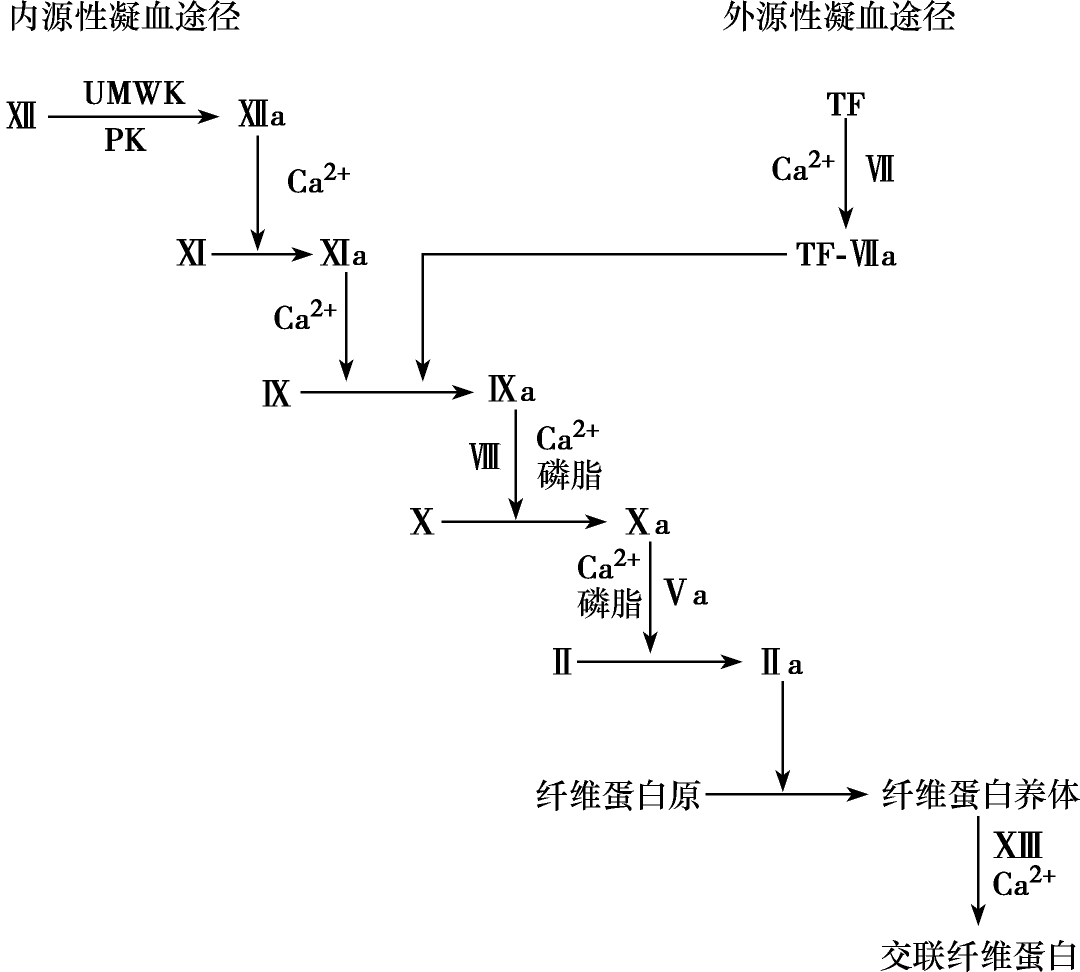
\includegraphics[width=3.79167in,height=3.32292in]{./images/Image00192.jpg}
 \captionsetup{justification=centering}
 \caption{内源和外源性凝血途径}
 \label{fig34-1}
  \end{figure} 

\section{【出血性疾病的分类】(表\ref{tab34-1})}

\section{【出血性疾病的一般诊断和鉴别诊断】}

对出血倾向的患者,首先应区分是局部因素还是出血性疾病,凡多部位或多系统出血,自发性深部组织或关节腔出血,与创伤不相吻合的大出血或创面经清创,缝合仍出血不止,拔牙或小手术后出血不止应考虑出血性疾病。患者的出血特点、出血诱因、基础疾病和家族史等有助于做出诊断和鉴别诊断。应结合病史、体检和实验室检查综合分析。病史应注意询问出血部位(皮肤、黏膜、牙龈、鼻腔、关节腔、深部组织、尿液、月经),出血程度及出血诱因,家族中有无同类病史。

以自发性皮肤、黏膜的紫癜为主要的临床表现者,是血管或血小板出血的特征。凝血机制异常型的出血主要以外伤后深部组织的出血与血肿形成,或发生非损伤性关节积血,或皮肤黏膜持续渗血为特征。如患者有自发的广泛或局部(皮肤、黏膜、关节、肌肉等)的出血,或外伤、手术后出血不止,或兼有家族成员中易出血史,提示有止血与凝血机制异常的可能性。

遗传性止血与凝血机制异常有自幼出血史及亲属中有出血异常;获得性者多发生在成年期以后,有原发病病史的或药物(或化学物品)接触史。通过病史、家系调查及特殊检查,初步确定为先天性、遗传性或获得性,对先天或遗传性疾病,应进行基因及其他分子生物学检测以明确病因。

出血性疾病实验检查项目繁多(表\ref{tab34-2}),应根据筛选、确诊及特殊试验的顺序进行。

\begin{longtable}{c}
 \caption{出血性疾病的分类}
 \label{tab34-1}
 \endfirsthead
 \caption[]{出血性疾病的分类}
 \endhead
 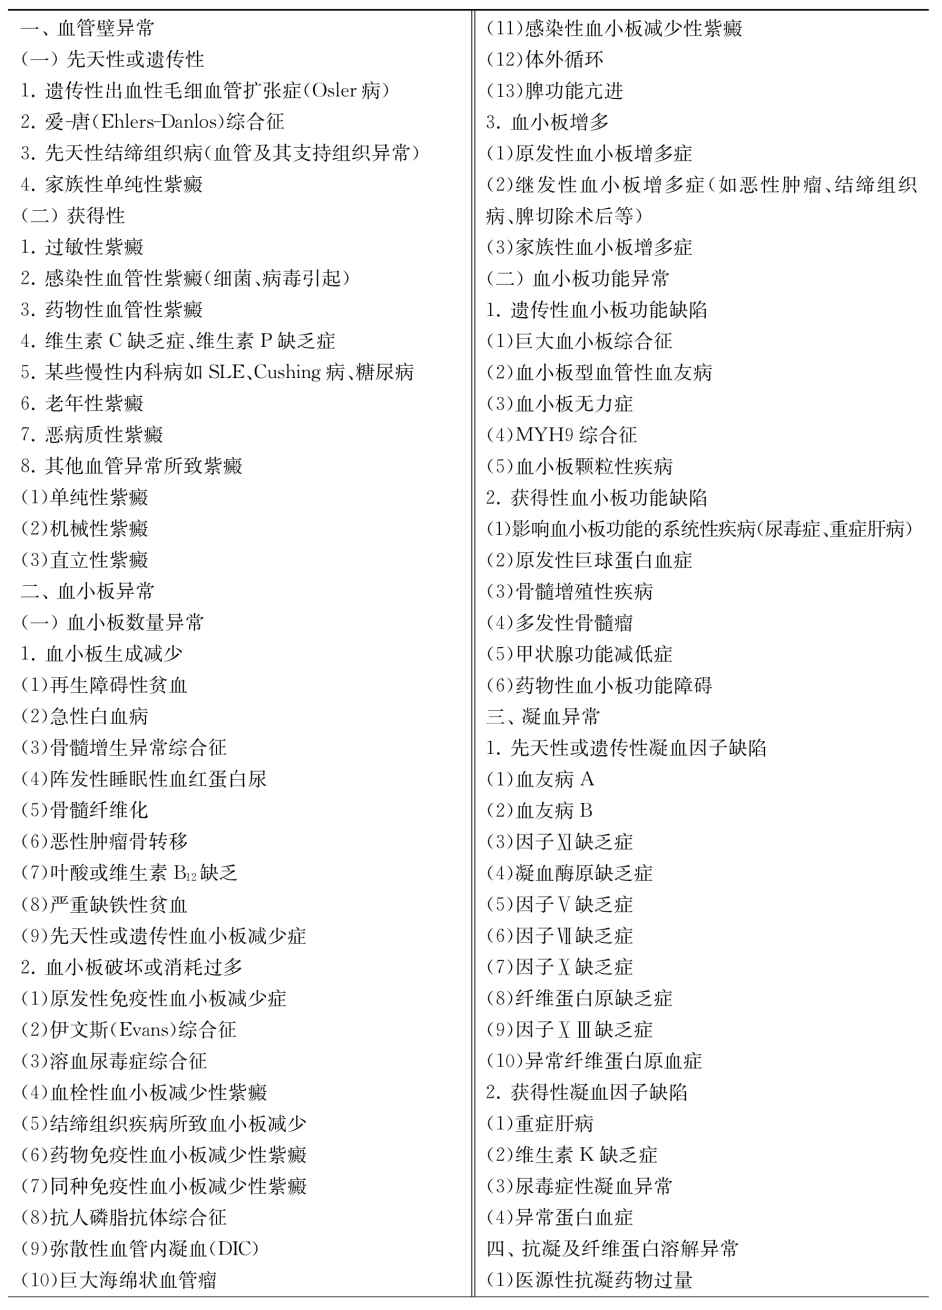
\includegraphics[width=\textwidth,height=\textheight,keepaspectratio]{./images/Image00193.jpg}\\
 
\includegraphics[width=\textwidth,height=\textheight,keepaspectratio]{./images/Image00194.jpg}
 \end{longtable}

\begin{longtable}{c}
 \caption{常用止血与凝血机制的实验室检查}
 \label{tab34-2}
 \endfirsthead
 \caption[]{常用止血与凝血机制的实验室检查}
 \endhead
 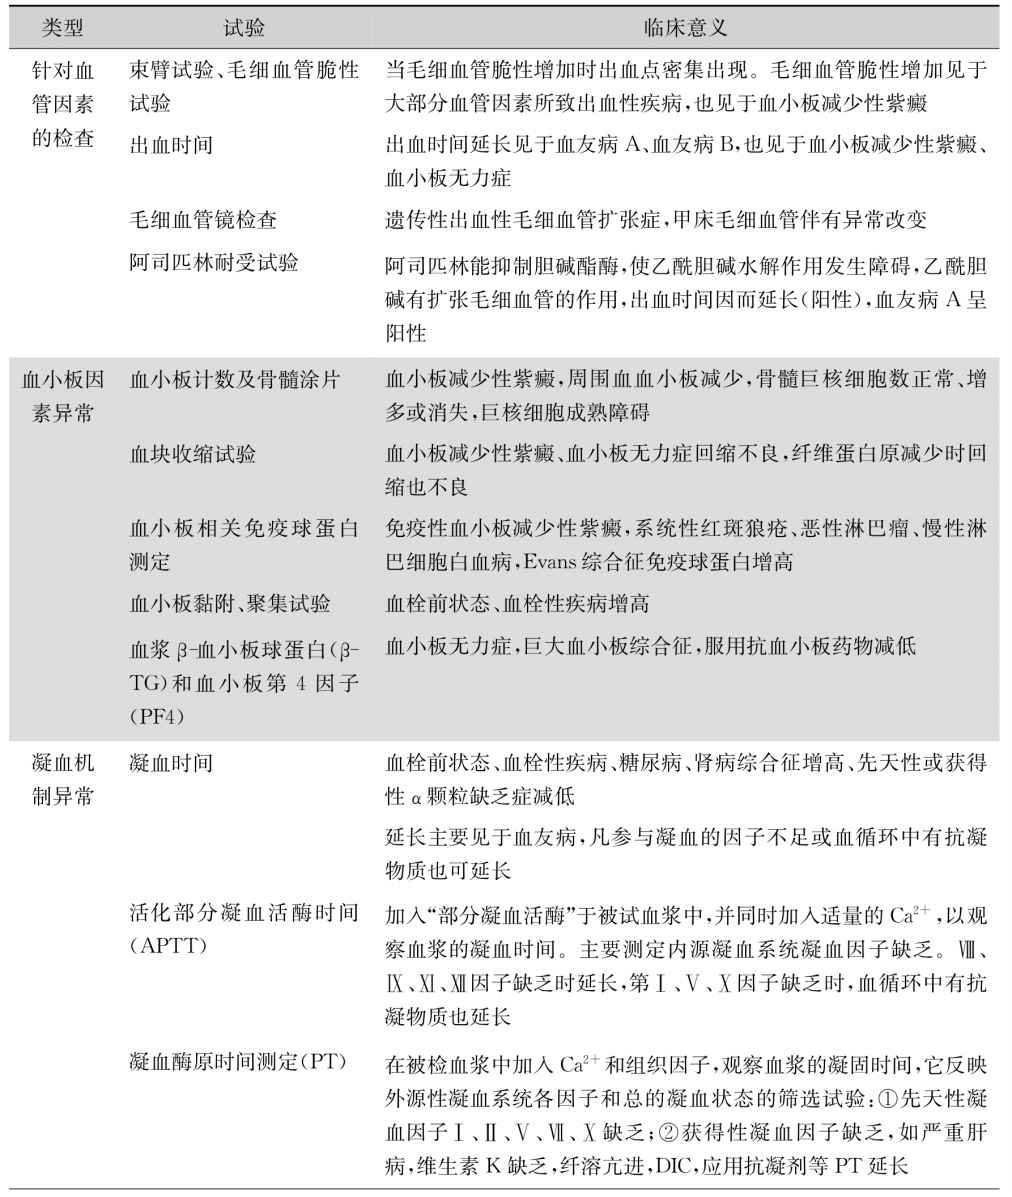
\includegraphics[width=\textwidth,height=\textheight,keepaspectratio]{./images/Image00195.jpg}\\
 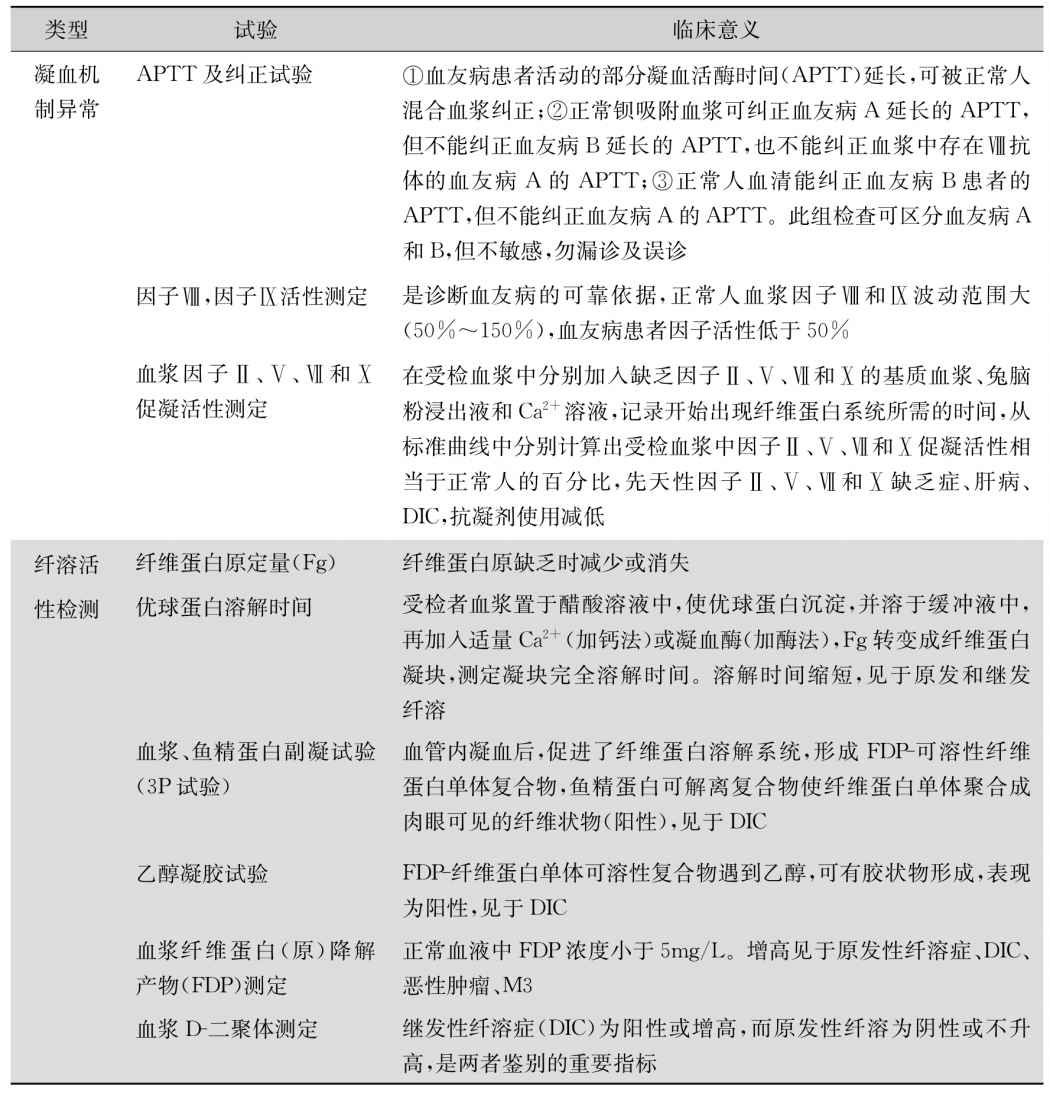
\includegraphics[width=\textwidth,height=\textheight,keepaspectratio]{./images/Image00196.jpg}
 \end{longtable}

\protect\hypertarget{text00264.html}{}{}

\section{115 紫癜}

紫癜通常为血管因素及血小板因素所致出血性疾病的主要表现,约占出血性疾病总数的1/3。凝血机制异常所致出血性疾病虽也有紫癜的出现,但非显要的体征。

血管因素所致出血疾病,临床表现以瘀点、瘀斑为特征,通常少有血肿发生;实验室检查出血时间、束臂试验、阿司匹林耐受试验及毛细血管镜检查等呈阳性。血小板因素所致出血性疾病,自发性瘀点、瘀斑远较血管外因素和血管因素严重,并可有胃肠道、阴道出血,内腔出血提示预后不良,颅内出血常为致死原因之一;实验室检查血小板计数、出血时间、血块回缩试验、束臂试验等有一项或多项异常。

\subsection{115.1 血管壁的异常}

血管因素所致的出血性疾病按病因的不同分为先天性(遗传性)与获得性两种类型。

\subsubsection{115.1.1 先天性(遗传性)}

\paragraph{一、遗传性出血性毛细血管扩张症}

本病临床少见,也称Rendu-Osler-Weber病。若固定在一部位的皮肤或黏膜有毛细血管扩张,伴有固定在一部位皮肤或黏膜的反复出血时,应怀疑本病的可能性。本病是显性常染色体遗传疾病,男女均可罹患。80\%病例可有阳性家族史。主要病变为累及小动脉和毛细血管,形成毛细血管扩张。毛细血管扩张可分布于全身各处,但以面部、上肢的皮肤,口腔、鼻及消化道黏膜较为常见。凡有毛细血管扩张的部位,均可出血。故本病也有并发消化道出血者。毛细血管镜检查甲床可见扩张的毛细血管袢,其余实验室检查无异常发现。

毛细血管扩张的特点为:形态大小不一,颜色紫红,可为点状、结节状或蜘蛛样改变。直径1~3mm,压之退色。临床上应与蜘蛛痣相区别,后者分布很少发生在腰部以下,也不见于黏膜,直径常超过3mm,大小形态较为一致,颜色颇鲜红。此外,本病局部表皮无过度角化征,可与角化性血管瘤(红痣)相区别。

本病的诊断根据是:①同一部位反复出血;②典型的毛细血管扩张;③阳性家族史。

\paragraph{二、爱-唐综合征}

本综合征为一种遗传性间叶发育异常的疾病,也称Ehlers-Danlos综合征,临床上罕见,国内曾有少数病例报告。本综合征的特点为:①皮肤弹性过强;②关节过伸;③轻微外伤或关节过伸可引起出血。

\paragraph{三、遗传性家族性单纯性紫癜}

本病国内尚无报告。临床特点为:①自发性瘀斑;②有阳性家族史;③多数病例止血带试验阳性,其他止血及凝血机制试验正常。

\subsubsection{115.1.2 获得性}

\paragraph{一、过敏性紫癜}

患者多数为儿童或青年,发病在20岁以下者占半数以上,无明显性别差异。大多数病例找不到明确病因,可能的病因较多。较重要的为:①感染:值得注意的病原菌为溶血性链球菌、病毒,部分患者发病前1~3周有明确的呼吸道感染史;②药物:如磺胺类、水杨酸钠、奎宁等;③食物:如虾、蟹等;④其他:如植物花粉、寄生虫感染、昆虫叮咬等。这些因素可能具有过敏原的作用,使人体发生过敏反应。发病高峰在冬春季节。

本病特点为皮肤紫癜伴有其他渗出性病变,而实验室止血及凝血机制检查无明显改变。

根据临床表现分为单纯型(紫癜型)、腹型(Henoch型)、关节型(Schonlein)型、肾型、混合型。皮肤症状见于所有病例,而腹部症状,关节痛仅见于半数以下。如以持续性显微镜下血尿为肾损害的最低诊断条件,则肾损害占46.6\%。皮肤表现为对称性各种各样的皮疹、小型荨麻疹或淡红色圆形丘疹,多伴有轻度痒感,于数小时内其色增深,变为各种形态的红斑,或经数小时后红斑的中心发生点状出血,出血点的红晕于短期内消失,与一般紫癜不易区别。皮疹孤立存在或融合成片,几乎均见于四肢及臀部,而以近关节处的伸侧为多,在面部及躯干甚少。关节症状可自轻微的疼痛乃至明显的红、肿、热、痛,可单发或多发。紫癜未出现时,可误诊为风湿性关节炎,但过敏性紫癜多有过去紫癜和过敏史。腹部症状临床表现无特异性,腹痛剧烈而部位多变、腹部体征轻微,是其临床特点之一。表现为不同程度的腹痛甚至绞痛,有的病例腹痛先于皮肤紫癜,可类似外科急腹症,但腹肌强直较轻,无固定压痛点,血中白细胞数不增多而嗜酸性粒细胞增多,大致可除外外科急腹症,腹型过敏性紫瘫患者的胃肠黏膜广泛散在大小不一的出血点和雪花状多发性溃疡。肾损害以血尿表现为主,少数病例发生局灶性或慢性肾炎。实验室检查血小计数正常,出血时间、凝血时间、血浆凝血酶原时间及血块回缩试验均正常;血中嗜酸性粒细胞计数多增加;骨髓巨核细胞计数与分类均正常。多数病例束臂试验阳性。

过敏性紫癜的诊断主要根据:①上述的感染、药物或食物等过敏史,但绝大部分病例查不出明确的致敏原;②皮肤紫癜呈对称性分布,罹患部位主要为四肢与臂部,尤以四肢伸侧,并多伴有关节、腹部及肾脏的症状;③上述的实验室检查所见。

\paragraph{二、症状性非血小板减少性紫癜}

症状性非血小板减少性紫癜系一继发的现象,其原发病的病象或致病因素十分明显,束臂试验多呈阳性。紫癜仅为原发病伴随症状之一,无明显的关节与腹部症状,据此可与过敏性紫癜相区别。血小板计数一般正常,可与血小板减少性紫癜相区别。此型紫癜可见于:

\subparagraph{(一)感染}

许多感染都可引起紫癜,虽可伴有血小板减少,但血小板计数正常者更为多见。在亚急性细菌性心内膜炎时,紫癜通常起于细菌性栓塞。脑膜炎双球菌败血症的紫癜也可引起细菌性栓塞,但主要则为毒素对毛细血管的损害。实验证明肺炎双球菌的自身溶解产物可引起紫癜。其他可引起非血小板减少性紫癜的感染尚有伤寒、流感、猩红热、肾病综合征、出血热、钩端螺旋体病、回归热、鼠疫、结核病、疟疾、麻疹、白喉、恙虫病、斑疹伤寒和各种细菌所致败血症等。感染并发紫癜时常提示病情较重。出血性麻疹的紫癜常在皮疹之前出现,易被误诊为其他疾病。

\subparagraph{(二)化学性因素}

碘化物、颠茄、阿托品、奎宁、青霉素、普鲁卡因、铋剂、汞剂、非那西丁、水杨酸制剂、水合氯醛及其他安眠药等化学物品,均可引起非血小板减少性紫癜。

\subparagraph{(三)维生素C缺乏症}

维生素C缺乏症(坏血症)在国内未见有成年人病例报告,但曾有小儿病例报告。本病的诊断可根据:①病史方面有食物中长期缺乏新鲜蔬菜与水果,或有消化不良、吸收障碍和需要增加等病史;②出血部位见于皮肤、肌肉和黏膜,牙龈红肿出血为本病特征;③四肢肿胀、压痛,出现坏死性肋骨串珠;④贫血;⑤假性瘫痪;⑥束臂试验阳性;⑦血浆维生素C测定含量降低;⑧补给维生素C后症状迅速好转;⑨X线征象是诊断维生素C缺乏症的重要依据,主要X线征有:长骨骺线增厚、骨膜下出血、骺线外展形成横突骨刺、全身性骨质疏松,尤其重要的是骨骺成骨中心脱钙,密度减低,围绕有密度增加的圈环。

\subparagraph{(四)某些慢性内科病}

有些慢性内科病可并发非血小板减少性紫癜,文献报道有慢性肾炎、肝功能不全、糖尿病等。

\subparagraph{(五)暴发性紫癜}

此型紫癜分两型。一型最常见于脑膜炎双球菌败血症,也称为华-弗(Waterhouse-Friderichsen)综合征。患者往往于短期内因中毒性休克而危及生命。华-弗综合征一般有下列五项临床特点:①突然发病;②短期内全身出现广泛性瘀点和瘀斑,并有迅速发展的倾向;③伴有严重周围循环衰竭,脉搏弱而速,血压显著下降,呼吸急促,面色苍白,口唇发绀;④瘀斑、脑脊液或血液细菌检查或培养阳性;⑤如抢救不及时可于短期内死亡。尸检可发现一侧或双侧肾上腺严重出血。目前认为暴发性紫癜与弥散性血管内凝血有关。此型暴发性紫癜可被误诊为急性原发性血小板减少症,但后者并无周围循环衰竭、发热与虚脱状态。

另一型暴发性紫癜可能是许兰-亨诺综合征的一种变异型。虽然死亡率也很高,但发病不如上述一型之急,且病程较长(2~7天)。这是一种罕见病,主要见于小儿。多发生于急性感染疾病时(尤其是猩红热),在感染过程中并发严重而往往致死的急性血管炎(vasculitis)、广泛性梗死及组织坏死,并有弥散性血管内凝血,酷似Schwartzman现象。尸检可见坏死性血管炎(necrotizing
vasculitis)及血栓形成。透明血栓在肾脏明显,腔静脉及髂静脉也有血栓形成。临床特点:起病急骤,寒战高热,循环衰竭,对称性皮肤紫癜和明显的皮肤与皮下组织的炎症性血管炎及坏死,黏膜也可出血,最后可出现出血性休克,中枢神经系统症状,甚至发生昏迷。实验室特点为:血小板计数正常或减少,第Ⅷ、Ⅴ因子减少,抗凝血酶及纤维蛋白溶酶含量增加。此型暴发性紫癜应与血栓性血小板减少紫癜相区别。前者溶血较为罕见,中枢神经系统症状为晚期症状,且中枢神经系统症状一经出现则呈不可逆性,皮肤与皮下组织有坏死性血管炎。后者溶血常见,且程度严重,反复出现神经精神症状,组织学检查无血管炎症性改变。

\paragraph{三、老年性紫癜}

老年人皮肤发生高度的老年性退行性变时,组织变松弛,毛细血管壁脆性增加,致毛细血管与小血管稍受不经意的轻微外伤,即引起破裂溢血而形成紫癜。出血部位多见于手、足、前臂的伸侧与桡侧以及上臂较大静脉和静脉分布之处。患者常无自觉症状,维生素C治疗无效。

\paragraph{四、恶病质性紫癜}

恶病质患者由于营养缺乏,皮肤萎缩,皮下脂肪消失,皮肤毛细血管受轻度外伤而易发生紫癜。

\paragraph{五、其他血管异常所致紫癜}

这组疾病的共同特点为:①大多数有紫癜或瘀斑,黏膜出血极其少见;②病因和发病机制有待阐明;③止血及凝血机制检查仅有束臂试验阳性,有些束臂试验也呈阴性。

\subparagraph{(一)单纯性紫癜}

此型紫癜经过和缓而较为慢性,患者几乎全为女性,尤常发生于月经期间。临床表现有下列特点:无外伤或其他诱因而不时出现皮肤瘀斑或瘀点,但无黏膜出血;患者无家族性易出血;血液学检查无明显的改变。

\subparagraph{(二)机械性紫癜}

当患者发作强力的肌肉收缩(例如百日咳发作)或惊厥时,或受止血带的长时间压迫时,可使受压迫部位的皮肤毛细血管发生破裂、溢血而形成紫癜。出血通常发生于头部、颈部及上肢。

\subparagraph{(三)直立性紫癜}

有些人在长期站立之后,可在下肢皮肤出现紫癜,可能为毛细血管壁脆弱所致。

慢性充血性心力衰竭患者可在下垂的肢体(下腿、足部)发生紫癜,这是由于静脉压升高与低氧血症所致的局部毛细血管通透性增加所引起。

\subsection{115.2 血小板的异常}

血小板在止血过程中占很重要的地位。血小板异常所致出血常由于血小板计数减少、血小板功能异常。其中以血小板计数减少为较常见的出血原因。

临床上要注意假性血小板减少。这是由于血液中存在抗凝剂依赖性或不依赖性的凝集素引起血小板凝集而发生假性血小板减少。患者常无出血倾向,通过反复多次血小板计数、更换抗凝剂、血涂片观察血小板分布可以诊断。

继发性血小板减少性紫癜发病数远较原发性者为多。继发性血小板减少性紫癜是指在有明确病因或某些疾病基础上发生的血小板减少。血小板减少伴有下列征象时,应考虑为继发性:①发病前有用药物史;②淋巴结肿大、明显的脾大及骨骼压痛;③发热;关节、肌肉痛;④失血量不多而贫血较重;⑤血沉加快;⑥骨髓穿刺涂片可发现:再生障碍性贫血、白血病及骨髓异常细胞浸润(多发性骨髓瘤、骨转移癌)等;⑦脾脏切除后作病理学检查,可发现引起血小板减少的病因。

\subsubsection{115.2.1 血小板生成减少}

血液病引起血小板生成减少性紫癜者常见,尤其是急性白血病、再生障碍性贫血、脾功能亢进、非霍奇金淋巴瘤等。此外叶酸或维生素B\textsubscript{12}
缺乏,严重缺铁性贫血、可导致骨髓造血功能抑制的物理、化学因素、严重感染、药物等也可导致血小板生成减少。

出血是急性白血病常见症状之一,多见于皮下、牙龈、口腔、鼻黏膜、眼底及中枢神经系统等部位。其中尤以颅内出血最为严重。如患者皮肤与黏膜出血,同时有剧烈头痛、恶心、失眠和烦躁不安,提示颅内出血的可能性。急性白血病出血原因主要由于血小板减少所致,此外尚有纤维蛋白溶解,凝血酶原减少和白血病细胞浸润使小血管破裂及弥散性血管内凝血等因素。

先天性血小板减少性紫癜少见,系婴儿疾病,国内仅有少数病例报告。

周期性血小板减少症罕见,国内只有个案报告。综合报告表明女性为男性的2倍,平均发病年龄女性为28岁,男性为52岁。血小板数变化周期为20~40天,平均30天。女性周期通常与月经一致,来潮时血小板数最低。血小板减少时可出现瘀点、瘀斑、鼻出血、胃肠出血、月经过多,甚至子宫大出血等,一般持续6~7天。病因尚未明了。对有周期性出血的患者须注意本病的可能性。

\subsubsection{115.2.2 血小板破坏或消耗过多}

\paragraph{一、原发免疫性血小板减少症}

原发免疫性血小板减少症(primary immune
thrombocytopenia,ITP)是比较常见的血液病,约占出血性疾病总数的1/3。在青壮年患者中,女性发病约为男性的2倍。综合国内文献,急性型占40\%,慢性型占60\%,年龄在20岁以下者占76\%,出血症状以鼻出血、皮下出血、牙龈出血、月经过多、血尿为多见,皮肤紫癜以四肢为主,黏膜出血则多见于鼻腔、口腔。

该病主要发病机制:①体液和细胞免疫介导的血小板过度破坏;②体液和细胞免疫介导的巨核细胞数量和质量异常,血小板生成不足。

ITP诊断是临床排除性诊断,其诊断要点如下:①至少2次检查血小板计数减少,血细胞形态无异常;②脾脏一般不增大;③骨髓检查:巨核细胞数增多或正常、有成熟障碍;④须排除其他继发性血小板减少症,如自身免疫性疾病、甲状腺疾病、药物诱导的血小板减少、同种免疫性血小板减少、淋巴系统增殖性疾病、骨髓增生异常[再生障碍性贫血(AA)和骨髓增生异常综合征(MDS)]、恶性血液病、慢性肝病、脾功能亢进、血小板消耗性减少、妊娠血小板减少、感染等;排除假性血小板减少以及先天性血小板减少等;⑤诊断ITP的特殊实验室检查:血小板抗体的检测和血小板生成素(TPO)水平检测。

ITP按疾病发生的时间及其治疗情况分期:

\subparagraph{(1)新诊断的ITP:}

指确诊后3个月以内的ITP患者。

\subparagraph{(2)持续性ITP:}

指确诊后3~12个月血小板持续减少的ITP患者。包括没有自发缓解的患者或停止治疗后不能维持完全缓解的患者。

\subparagraph{(3)慢性ITP:}

指血小板减少持续超过12个月的ITP患者。

\subparagraph{(4)重症ITP:}

指PLT<10×10\textsuperscript{9}
/L,且就诊时存在需要治疗的出血症状或常规治疗中发生新的出血症状,且需要采用其他升高血小板药物治疗或增加现有治疗的药物剂量。

\subparagraph{(5)难治性ITP:}

指满足以下3个条件的患者:①脾切除后无效或者复发;②仍需要治疗以降低出血的危险;③除外其他原因引起的血小板减少症,确诊为ITP。

急性型多见于儿童,发病急骤,黏膜与皮肤出血较重,发病前有呼吸道感染史。白细胞数轻度增多,据此可与脾功能亢进区别。红细胞数下降与失血程度相一致。鉴别诊断须注意再生障碍性贫血与急性非白血性白血病。本病白细胞计数不减少,骨髓巨核细胞正常或增多,为与再生障碍性贫血的主要鉴别点。与急性非白血性白血病的鉴别主要依据骨髓穿刺涂片检查或淋巴结活检。急性白血病患者周围血片和骨髓有原始幼稚的白血病细胞,本病多于几天至几周内出血停止,少数可迁延半年左右。急性型约1/5病例演变为慢性。

慢性型多见于成年人,病程数月至多年,出血现象常有反复发作与缓解。紫癜以下肢为多。女性患者常以月经过多而起病,经详细的血液学检查方发现为此病。有的病例可因牙龈出血而由口腔科首先发现。

颅内出血为ITP的严重并发症,但不常见,急性型较慢性型为多;头痛与头晕常为提示轻度颅内渗血的指征。患者可出现神志不清或谵妄,以致被疑为脑部感染。

急性型与慢性型ITP的鉴别诊断见表\ref{tab34-3}。

\begin{table}[htbp]
\centering
\caption{急性和慢性ITP的鉴别}
\label{tab34-3}
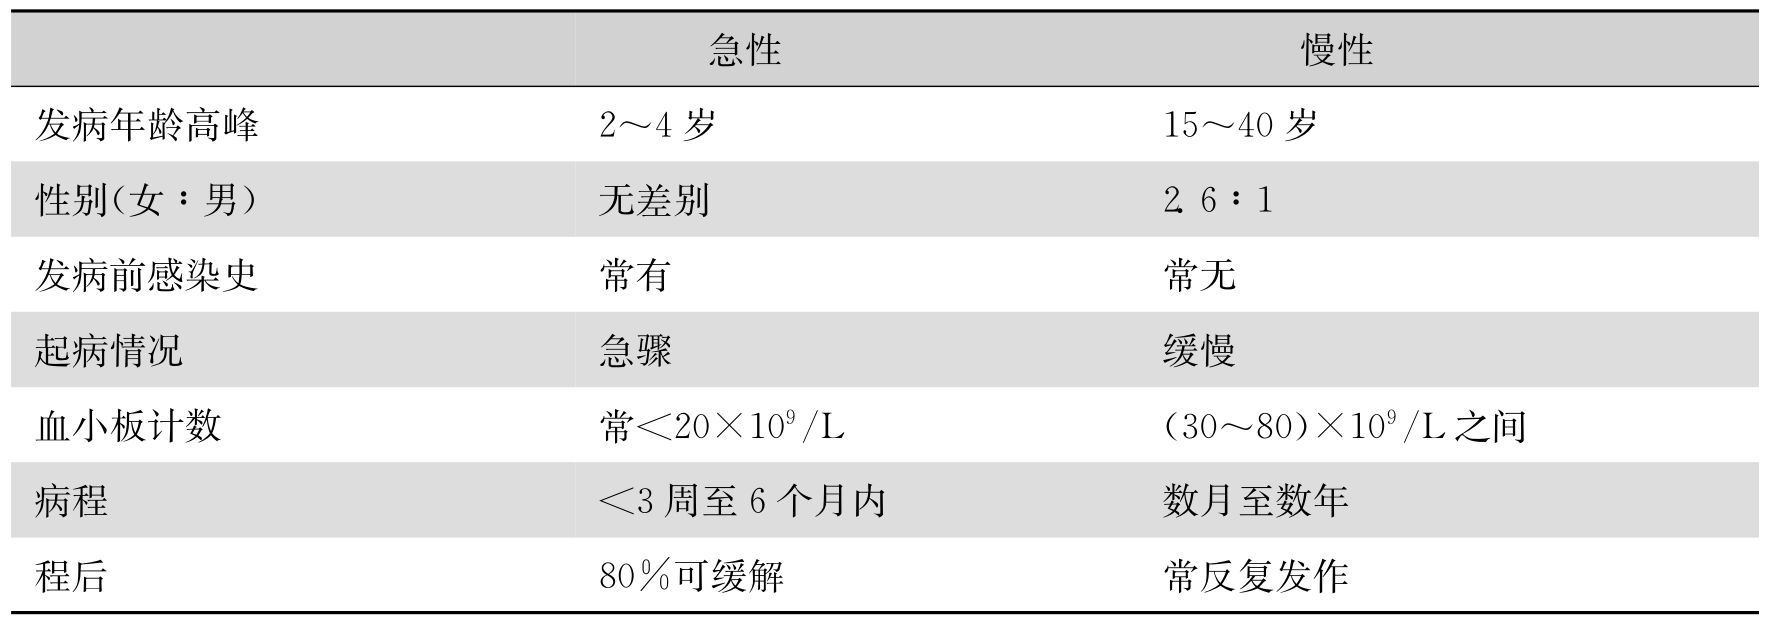
\includegraphics[width=5.875in,height=2.09375in]{./images/Image00197.jpg}
\end{table}

\paragraph{二、伊文斯(Evans)综合征}

本综合征为同时或相继发生AIHA和ITP,以血小板减少起病而后发生AIHA为多。本综合征的诊断主要依据:①原发免疫性血小板减少症;②除外其他原因的溶血性贫血;③抗人球蛋白试验阳性。

血涂片无红细胞碎片,抗人球蛋白试验阳性和活体组织检查无毛细血管内血栓形成,可与血栓性血小板减少性紫癜区别。

有报道84例Evans综合征患者中50例同时出现AIHA及血小板减少,20例以血小板减少起病,14例以AIHA起病。34例出现第二种血细胞减少从而诊断为Evans综合征的患者从起病到诊断经过了2个月至22年。起病时3例患者伴有白细胞减少,7例为全血细胞减少。疾病进展过程中2例出现白细胞减少,6例出现全血细胞减少。

\paragraph{三、血栓性血小板减少性紫癜}

本病少见,凡临床表现有:微血管性溶血性贫血、血小板减少及中枢神经系统表现发热及肾功能损害五联症或仅前三项表现三联症的症状和体征,则提示本病的可能性。本病的典型表现是:①血小板减少性紫癜,出血时间延长,血块回缩不良;末梢血片红细胞碎片>2\%;②急性血管内溶血性贫血;③反复出现神经精神症状;④肾功能障碍;⑤高热,有时呈败血性热型;⑥轻度黄疸,肝、脾大;⑦有些病例周围血液中出现暂时性类白血病反应。患者多在数周之内死于惊厥、尿毒症或肺炎。也有少数病例有多年缓解者。皮肤、肌肉、淋巴结或骨髓活检可见动脉或毛细血管内有透明血栓形成。以外周血破碎红细胞为特征的微血管病性溶血性贫血(Coombs试验阴性)和消耗性血小板减少仍是TTP诊断必备的条件。

临床上将TTP分为特发性、家族性和继发性三大类。继发性因素包括HIV病毒感染、骨髓干细胞移植、妊娠、药物相关性、风湿免疫性疾患等。

本病有溶血性贫血和毛细血管内透明血栓形成,可与特发性血小板减少性紫癜区别。鉴别诊断上尚须注意与败血症、系统性红斑狼疮、Evans综合征相区别。本病因血培养始终阴性,抗生素治疗无效,溶血明显,不支持败血症。测定ADAMTS13活性可以帮助鉴别TTP与其他具有TTP样临床表现的血栓性微血管疾病。

\paragraph{四、结缔组织病所致的血小板减少}

血小板减少是系统性红斑狼疮(systemic lupus
erythematosus,SLE)主要并发症之一,发生率约为7\%~30\%,其中5\%~10\%的患者PLT严重减少(≤40×10\textsuperscript{9}
/L)。血小板减少性紫癜可为系统性红斑狼疮早期的主要表现,可被误诊为ITP。中山医学院曾报告有数例,早期仅表现为血小板性紫癜,无SLE多系统损害的任何表现,历经3~5年,最长者达8年才出现典型的SLE症状体征和实验室指标异常。对年轻女性兼有白细胞减少时应注意SLE并进行抗ds-NDA、抗DNA、抗SM、抗SS-A、抗SS-B脂抗体以及肝、肾功能检测。

抗磷脂抗体综合征主要临床表现为无菌性血栓形成、流产、血小板减少、皮肤瘀斑等。本病可为原发性与继发性。国内有少数病例报告。如发生于系统性红斑狼疮等基础上则为继发性。实验室检查血小板减少,抗心磷脂抗体IgG(+)。

\paragraph{五、药物免疫性血小板减少性紫癜}

国内报道引起血小板减少性紫癜的药物,有碘化物、奎尼丁、异烟肼、氯霉素、青霉素、碘胺类等,紫癜的发生和药量关系不大。发病前有用药史,停药后症状缓解,但虽再用小剂量,又可引起较重的反应而再现紫癜,可与特发性血小板减少性紫癜相区别。

\paragraph{六、感染性血小板减少性紫癜}

伤寒、副伤寒甲引起血小板减少性紫癜者国内有数例报告。紫癜大多发生于病程14~15天,其发生似与感染的轻重程度无关。

结核病引起的血小板减少性紫癜的发生率,国内两组病例报告分别为1.4\%与2.7\%。绝大多数发生于女性患者。紫癜的出现多表示结核病已达严重阶段。

恶性疟、间日疟、传染性单核细胞增多症、波状热、蛔虫病、亚急性感染性心内膜,病毒性肝炎引起血小板减少性紫癜者国内也有报告。

\paragraph{七、溶血性尿毒症综合征}

本综合征临床上少见,发病多见于2岁以下的小儿,但也可见于成人。其发病机制可能是由于体内单核-吞噬细胞系统对革兰氏阴性细菌的内毒素的去毒作用不全,以致出现全身弥散性血管内凝血所致。也有报告与病毒感染有关;也有认为是由于全身性或肾小球局限性脉管炎所致。也有报告发生于产后。

本综合征的临床特点是:①重度的微血管病性溶血性贫血伴有周围血出现异形红细胞如刺细胞,三角形、新月形、钢盔样红细胞或红细胞碎片;②血小板减少、凝血机制障碍,广泛性出血;③肾功能障碍;④中枢神经系统症状如抽搐、木僵或昏迷。此外,在疾病的早期,患者常有发热、上呼吸道症状、呕吐、腹泻、排黏液样或血腥臭大便等。

血小板减少甚常见,可能是由于血小板过多破坏所致。临床上本综合征常需与血栓性血小板减少性紫癜相鉴别。有人认为两者为同一种疾病,仅发病年龄有所不同,本综合征多见于小儿,预后稍好;血栓性血小板减少性紫癜多见于成人,预后较差。此外,从病理改变和临床经过也有助于区别,本综合征除了肾损害以外,其他器官损害较轻,病情恢复后一般无反复发作;血栓性血小板减少性紫癜,常伴有其他器官的严重损害,呈慢性反复发作过程。

\paragraph{八、其他原因所致的血小板减少性紫癜}

血小板减少偶见于甲状腺功能亢进症;短期内输入大量的血库藏血后,也可引起短暂的重度血小板减少持续数天之久,血小板减少的程度与输入的血量有关,可能因受血者血小板的浓度被库血稀释所致。此外尚有妊娠期血小板减少、输血后紫癜、肝素诱导的血小板减少性紫癜、周期性血小板减少症、低温麻醉所致血小板减少等因素导致血小板减少。

\subsubsection{115.2.3 血小板增多}

无原发病的血小板增多伴出血现象,称为原发性出血性血小板增多症。

血小板增多伴出血现象还可见于真性红细胞增多症、慢性粒细胞型白血病、急性出血或溶血、恶性肿瘤、骨髓纤维化及脾切除术后等,这统称为继发性出血性血小板增多症。患者血小板计数超过正常(一般在1000×10\textsuperscript{9}
/L以上),并伴有出血现象,以黏膜出血(尤其是胃肠道出血)为主。本病血小板数虽然增多,但活动性凝血活酶生成迟缓,可能由于血小板功能异常,具有血小板病的异常特征。活动性凝血活酶生成迟缓为出血原因之一。偶尔血小板增多也可引起血栓形成的倾向。

\subsubsection{115.2.4 血小板功能异常}

血小板功能异常包括遗传性与获得性,出血原因主要由于血小板功能障碍而并非由于血小板数减少所致。出血性血小板增多症的出血可能也与血小板功能障碍有关。获得性血小板功能异常包括影响血小板功能的系统性疾病(尿毒症、重症肝病)、浆细胞疾病(多发性骨髓瘤、原发性巨球蛋白血症等)、甲状腺功能减低症、药物性血小板功能障碍(如阿司匹林等)。

\paragraph{一、血小板无力症}

血小板无力症(thrombasthenia)又称Glanzmann病,是一种隐性常染色体遗传疾病。本病主要缺陷是血小板GPⅡb和(或)GPⅢa质或量的异常,原因为其基因突变,包括替代、缺失,插入等造成的错义、无义或移码突变。临床上罕见,国内有少数病例报告。本病的临床特点是:①多发性瘀斑及反复鼻出血多主要临床表现;②有家族出血病史;③血小板数正常;④出血时间延长;⑤血块回缩不良;⑥血小板黏附性异常;⑦患者富含血小板的血浆中加入ADP,血小板聚集速度缓慢(正常人血小板则迅速发生聚集);⑧胶原和肾上腺素均不能诱导患者的血小板发生聚集而对瑞斯托霉素聚集正常。

出血时间延长、血小板计数正常、血块回缩不良及血小板黏着性异常,DOADP胶原、肾上腺素均发生聚集,加瑞斯托霉素则聚集正常。是诊断本病的要点。

本病因血小板数正常而出血时间延长,需与甲型假性血友病区别。后者以出血时间延长为唯一的实验室阳性发现,可与本病区别。

\paragraph{二、巨大血小板综合征}

巨大血小板综合征(Bernard-Soulier
syndrome,BSS)为常染色体隐性遗传性疾病,发病机制为血小板膜糖蛋白(GP)Ⅰb/Ⅸ/Ⅴ减少或缺乏。其特征性表现包括出血时间延长,血小板减少,巨大血小板和不同程度的出血症状。外周血片可见为巨大血小板,血小板直径可达8~10μm。血小板对ADP、胶原和肾上腺素聚集正常,但瑞斯脱霉素不能诱导血小板聚集。本病需与ITP、MYH9综合征、血管性血友病及血小板无力症相鉴别。

\paragraph{三、MYH9综合征}

MYH9综合征为常染色体显性遗传性疾病,MYH9基因编码非肌性肌球蛋白重链ⅡA,其突变引起了MYH9相关性疾病,大多数MYH9基因的突变为误义突变并且影响了NMMHC-ⅡA的启动子或卷曲状结构域。患者表现为血小板巨大,血小板减少和中性粒细胞包涵体。部分患者在儿童期或成人期,出现感觉神经性听力丧失、白内障、和(或)肾小球肾炎的症状。

\protect\hypertarget{text00265.html}{}{}

\section{116 凝血机制异常}

凝血机制异常有下列三类原因:

(一)血浆凝血因子缺陷

(二)抗凝及纤维蛋白溶解异常

(三)复合性止血机制异常

\subsection{116.1 血浆凝血因子缺陷}

任何一种血浆凝血因子缺乏都可引起异常出血,但Ca\textsuperscript{2+}
和第Ⅻ因子则为例外。第Ⅻ因子缺乏临床上无出血现象。Ca\textsuperscript{2+}
下降达到引起出血症状水平之前,心血管系统与神经肌肉系统早已出现严重障碍。单独一种凝血因子缺乏见于遗传性异常;获得性异常则有多种凝血因子同时累及。各种凝血因子缺乏所致疾病见表\ref{tab34-4}分述于下。

\begin{longtable}{c}
 \caption{血浆凝血因子名称及其缺乏时所致疾病}
 \label{tab34-4}
 \endfirsthead
 \caption[]{血浆凝血因子名称及其缺乏时所致疾病}
 \endhead
 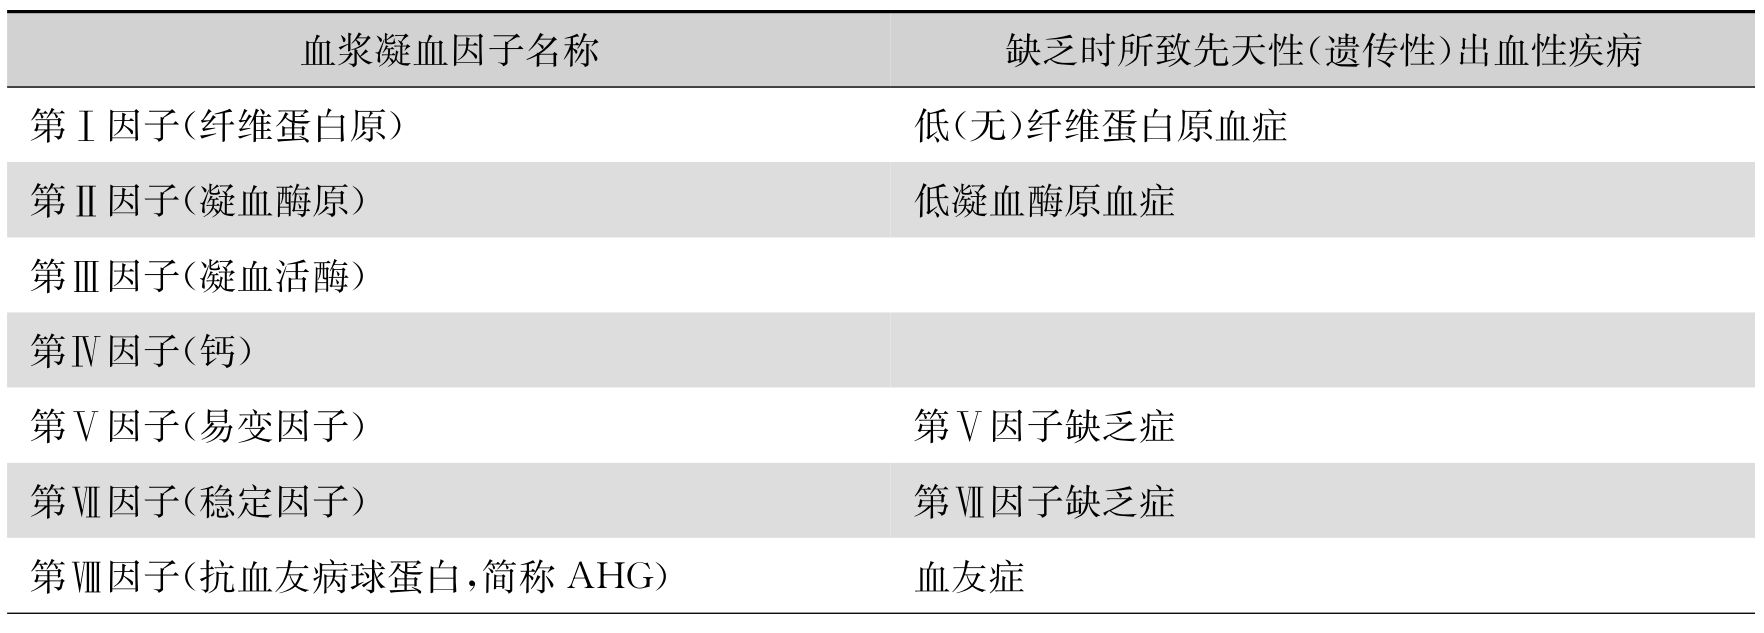
\includegraphics[width=\textwidth,height=\textheight,keepaspectratio]{./images/Image00198.jpg}\\
 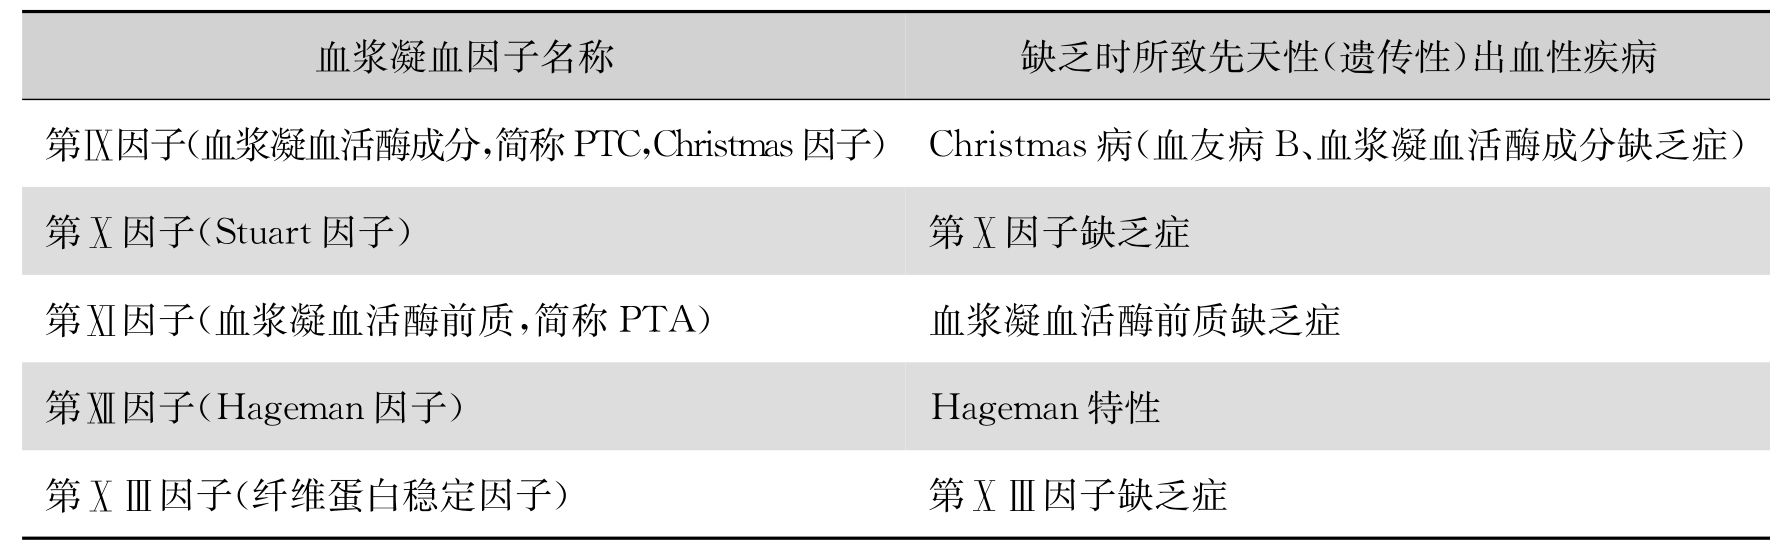
\includegraphics[width=\textwidth,height=\textheight,keepaspectratio]{./images/Image00199.jpg}
 \end{longtable}

\subsubsection{116.1.1 第一阶段凝血异常}

此类疾病表现为凝血过程第一阶段发生障碍,包括以下遗传性出血性疾病:血友病A(第Ⅷ因子缺乏症)、血友病B(第Ⅸ因子缺乏症)、第Ⅺ因子缺乏症及第Ⅻ因子(Hageman)缺乏症等。

此组出血性疾病的实验检查结果,有下列的共同特点,可与其他出血性疾病相区别:出血时间正常、全血凝血时间延长、血块回缩时间正常、血小板计数正常、凝血酶原时间正常、血浆纤维蛋白原含量正常、血钙含量正常、凝血酶原消耗不良、部分凝血活酶时间延长、凝血活酶生成纠正试验异常及束臂试验阴性。

上述出血性疾病实验室检查相互鉴别参考表\ref{tab34-5}和表\ref{tab34-6}\footnote{+:不正常;-:正常;±:轻度不正常,仅在严重时呈不正常}。

上述四种出血性疾病的相互鉴别,可依靠凝血酶原消耗纠正试验,或更敏感的凝血活酶生成纠正试验,见表\ref{tab34-7}\footnote{+:存在;±:小量存在;-:不存在}和表\ref{tab34-8}\footnote{*红细胞素有血小板第3因子作用}。

血友病是一组比较常见的先天性凝血因子缺乏而致凝血功能异常的出血性疾病,有以下特点:①幼年出现,持续终生,反复轻微外伤或小手术出血不止,甚至自发出血;②大关节,下肢关节及其附带肌群出血多见;③多有家族史并极少发生于女性;④临床仍以医院治疗为主。在男性人群中血友病A的发病率约为1/5000,血友病B的发病率约为1/25
000;血友病A占血友病患者80\%~85\%,血友病B占15\%~20\%。而女性血友病患者极其罕见。

\paragraph{一、血友病A}

血友病A又称遗传性抗血友病球蛋白缺乏症或FⅧ:C缺乏症,是一种X染色体连锁的隐性遗传疾病,发病多限于男性,而依赖女性传递。只有极个别情况下,当男性血友病者与女性带病者结婚时,其女儿可能罹患本病。因其致疾基因位于X染色体,由于男性只有一条X染色体,具有病变染色体的男性均为患者。而具有致病基因的女性临床上一般无症状,称为携带者。血友病患者与正常女性结婚所生的男孩均正常,女孩均为携带者。女性携带者与正常男性结婚所生的男孩为正常人或患者的几率各为50\%,所生女孩为正常人或携带者的几率各为50\%。

本病有四项临床特征:①家族出血史,多限于男性患病,自幼有易出血史;②轻微外伤引起迁延难止的出血;③反复出现关节积血或其他深部组织的血肿;④全血凝血时间(PT)延长及APTT延长。

典型病例自幼即有易出血的倾向,一般常人所能经受的轻度外伤(例如拔牙)即可使患者发生持久的出血。四肢与内脏皆可出血,但以关节、四肢等易受伤的部位为常见。

\begin{table}[htbp]
\centering
\caption{出血性疾病的初步试验与特殊试验}
\label{tab34-5}
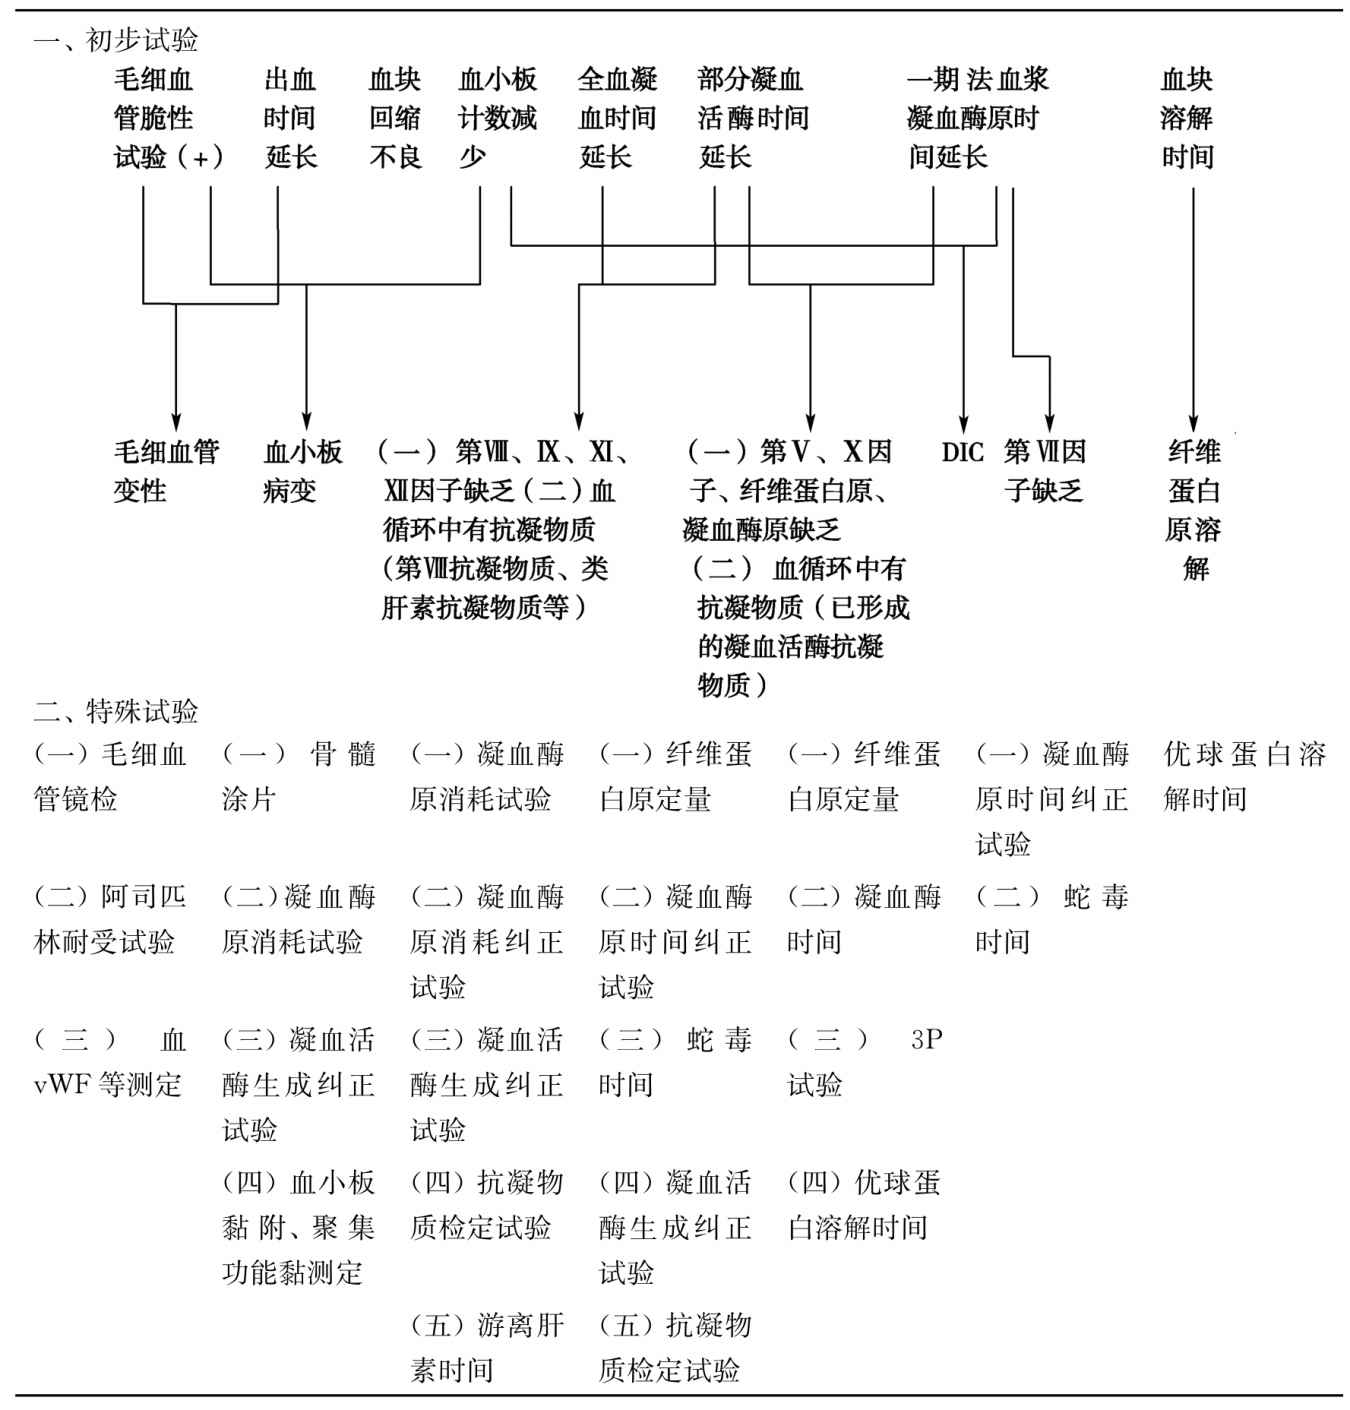
\includegraphics[width=5.91667in,height=6.17708in]{./images/Image00200.jpg}
\end{table}

轻型病例平素虽无明显的出血,但在外伤之后,甚至小手术后,可发生持久的出血,甚至危及生命,因此临床医生对此类疾病应予注意。如需进行手术的患者,过去有外伤易出血史,且家庭中也有类似的易出血者,在术前宜进一步作有关血友病的特殊检查,以明确诊断,如能作充分准备,可免发生意外。

血友病的确诊依靠下列的实验室检查:①全血凝血时间延长;②凝血酶原消耗不良;③血浆凝血酶原时间及出血时间正常;④活化的部分凝血活酶时间(APTT)延长;⑤作凝血酶原消耗纠正试验时,凝血酶原消耗不良能被吸附正常血浆纠正;⑥凝血活酶生成纠正试验(用患者吸附血浆),生成迟缓。血友病患者实验室检查的特点为活化的部分凝血活酶时间(APTT)延长,可被正常人混合血浆纠正。

\begin{table}[htbp]
\centering
\caption{止血及凝血机制异常的实验室鉴别诊断}
\label{tab34-6}
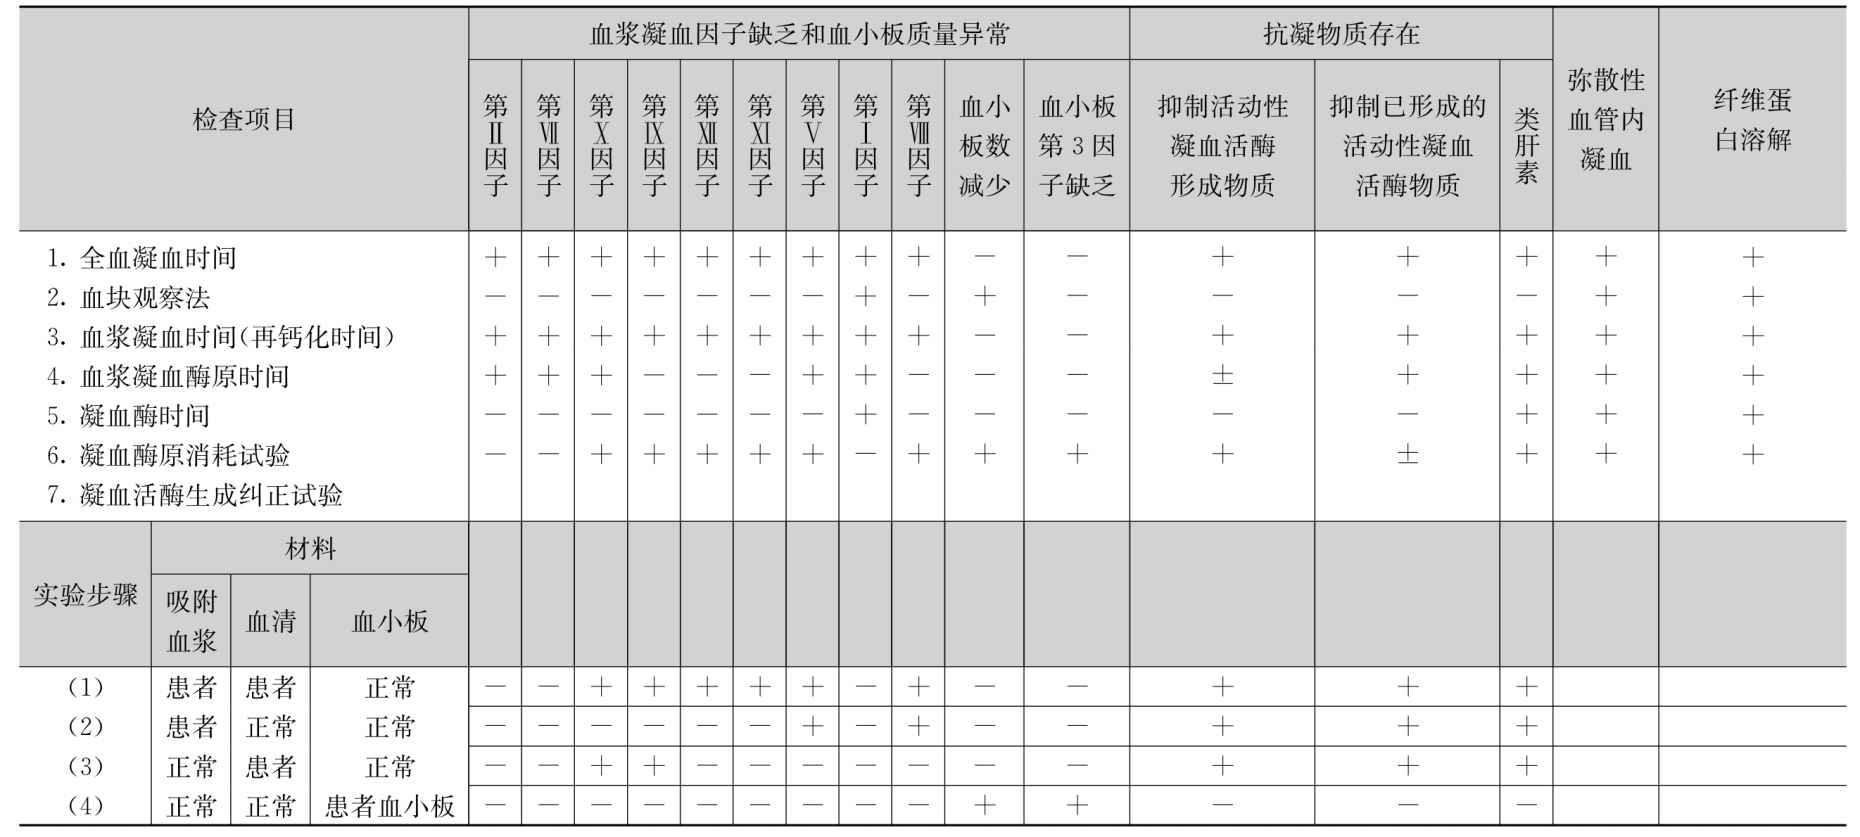
\includegraphics[width=8.80208in,height=3.95833in]{./images/Image00201.jpg}
\end{table}

\begin{table}[htbp]
\centering
\caption{各种血液制剂所含的因子}
\label{tab34-7}
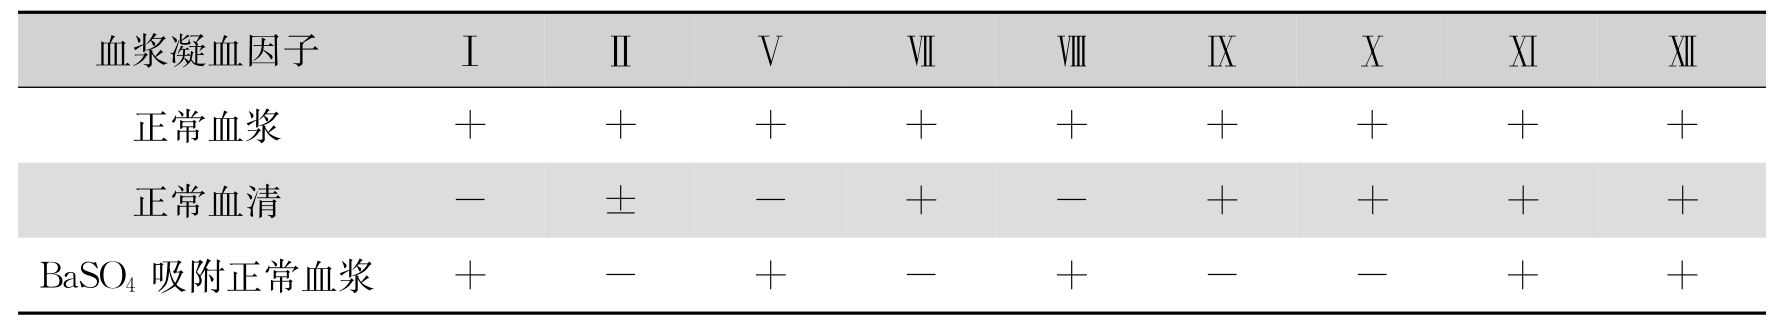
\includegraphics[width=5.9375in,height=1.07292in]{./images/Image00202.jpg}
\end{table}

\begin{table}[htbp]
\centering
\caption{凝血酶原消耗纠正试验}
\label{tab34-8}
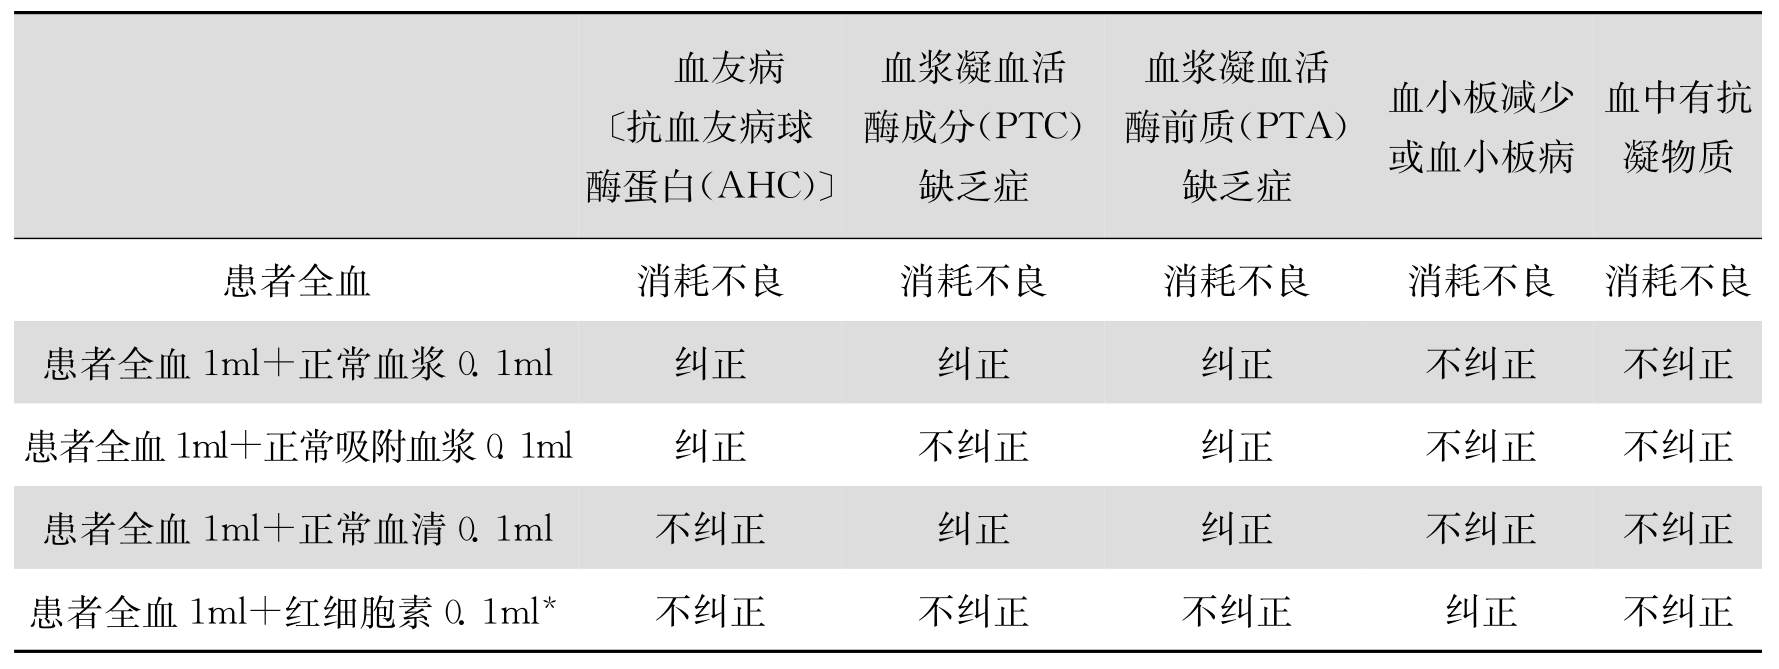
\includegraphics[width=5.91667in,height=2.21875in]{./images/Image00203.jpg}
\end{table}

对某些试验要有正确的评价。全血凝血时间延长见于重度第Ⅷ因子缺乏,凝血酶原消耗试验消耗不良见于中等度第Ⅷ因子缺乏,而部分凝血活酶时间延长及凝血活酶生成纠正试验生成迟缓,则见于轻度凝血因子减少状态,故后两项为较敏感的试验。个别极为轻型的病例,上述试验全在正常范围内,此时作血浆第Ⅷ因子定量测定可以确诊。Ⅷ因子或Ⅸ因子抗原及活性测定是诊断血友病的可靠依据,根据FⅧ或FⅨ的活性水平可将血友病分为3型(表\ref{tab34-9})。

\begin{table}[htbp]
\centering
\caption{血友病A/B临床分型}
\label{tab34-9}
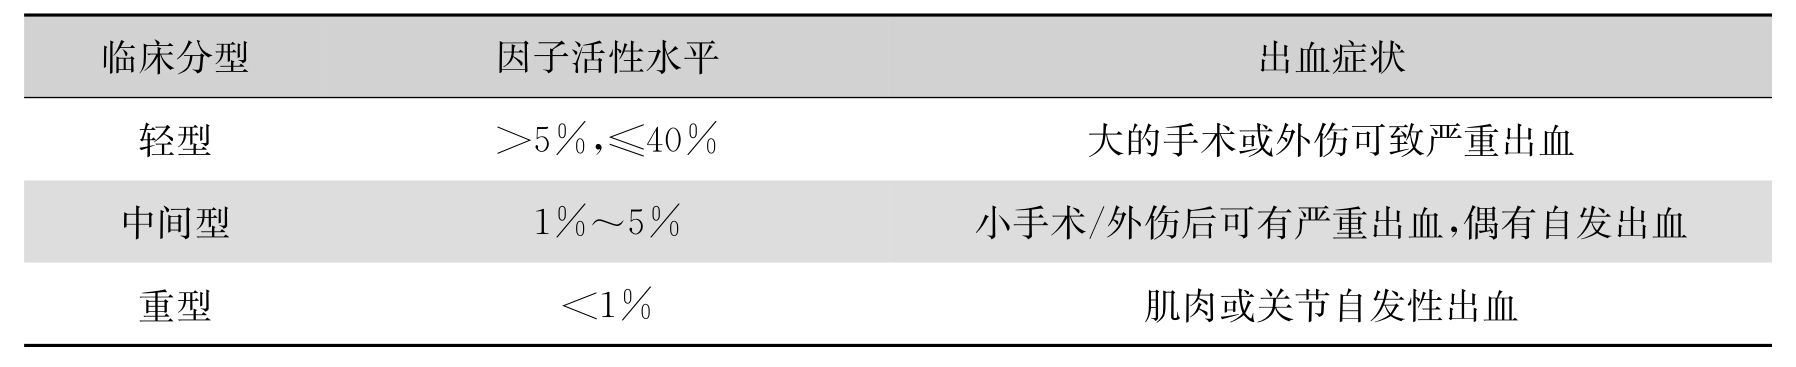
\includegraphics[width=5.97917in,height=1.21875in]{./images/Image00204.jpg}
\end{table}

中、重型血友病患者的诊断一般比较容易,轻型或亚临型血友病患者出血较轻或无出血史,APTT仅轻度延长,容易漏诊。不应仅凭APTT及纠正试验诊断血友病,而应根据凝血因子活性测定,有条件的,应同时测定凝血因子抗原。

血友病A要与血管性血友病,获得性血友病、遗传性FXI缺乏症等相鉴别。获得性因子Ⅷ缺乏症自幼无出血史,无家族病史,实验室检查患者循环血中不存在抗因子Ⅷ抗体。非血友病患者血中产生因子Ⅷ抑制物,临床称为获得性甲型血友病。

轻型血友病A与血管性血友病(VWD)的鉴别见表\ref{tab34-10}。

\begin{table}[htbp]
\centering
\caption{轻型血友病A与血管性血友病(vWD)的鉴别}
\label{tab34-10}
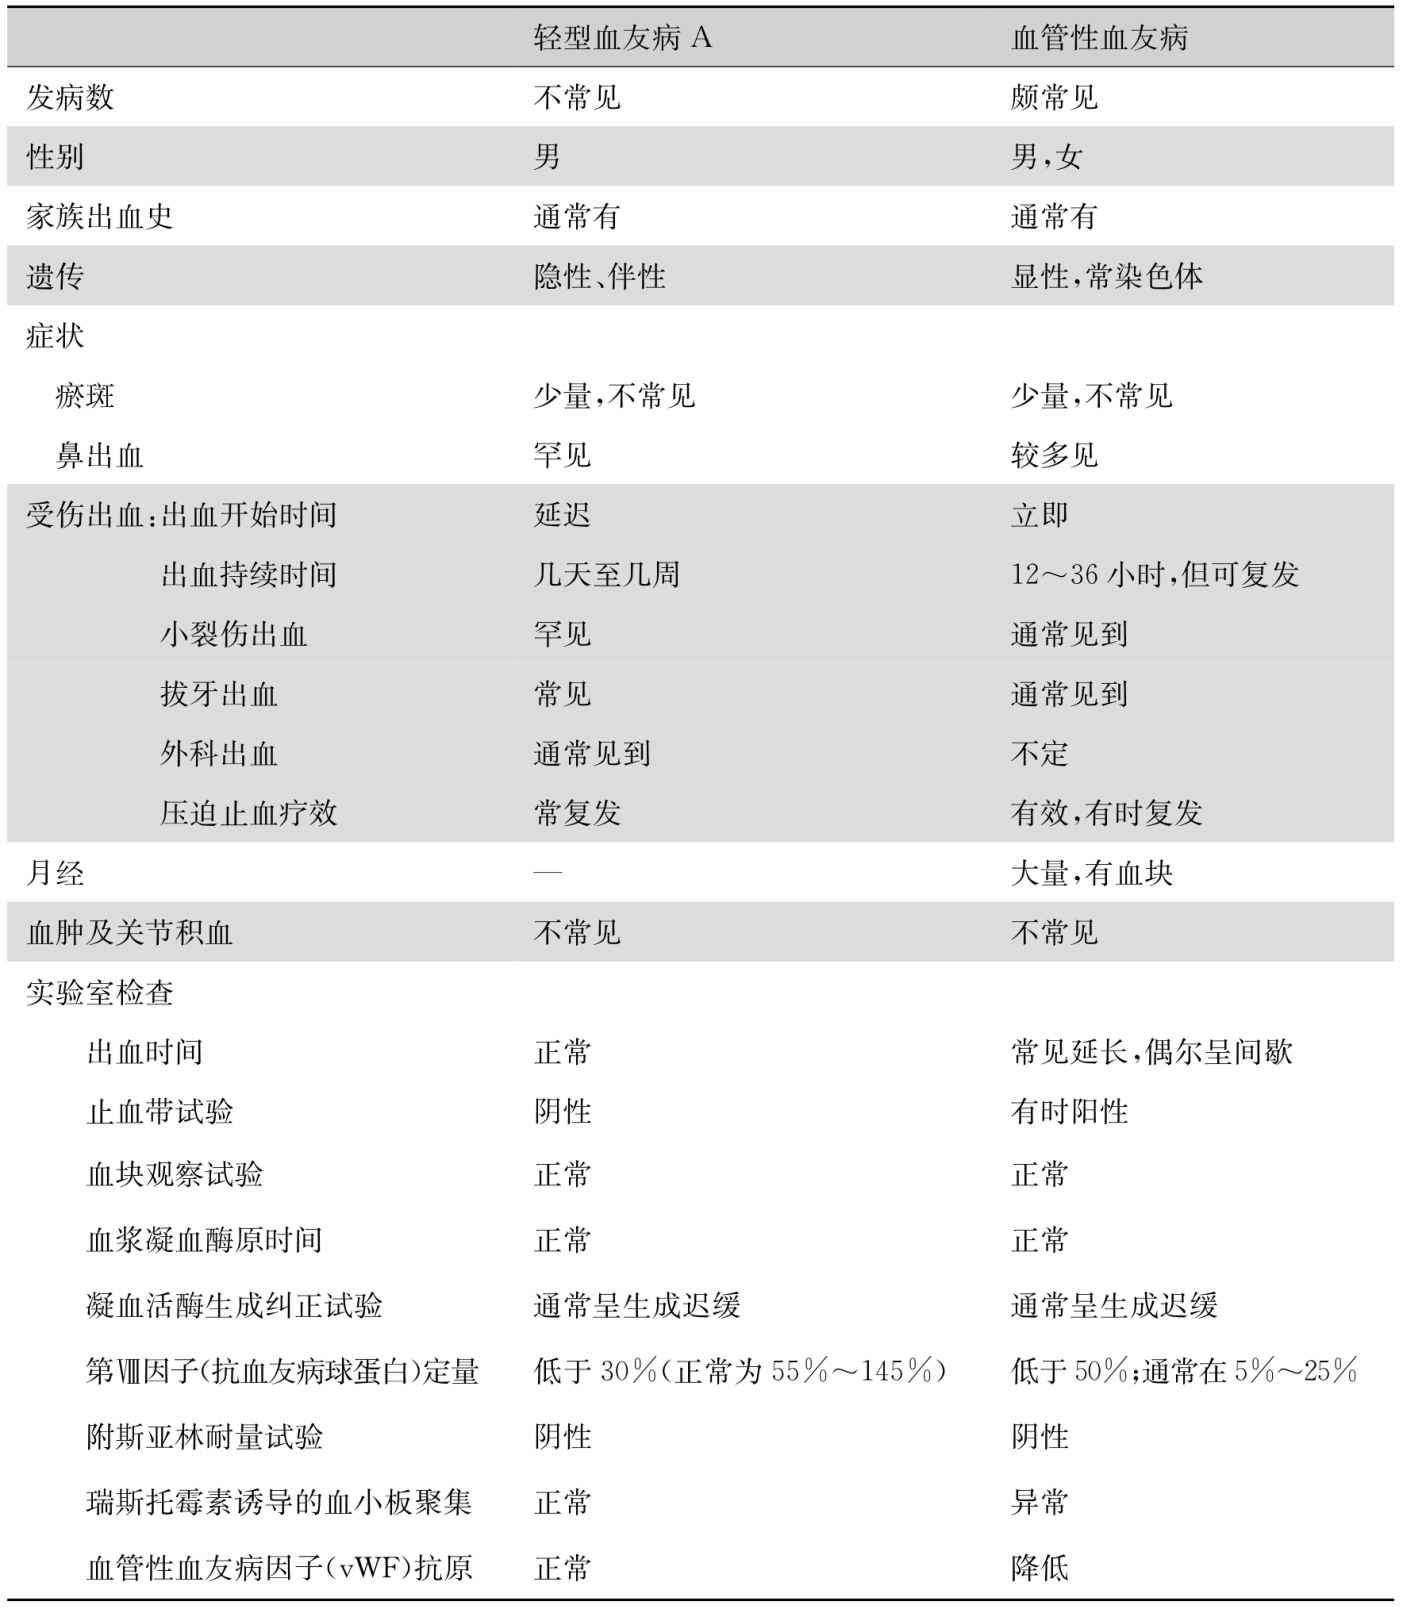
\includegraphics[width=5.88542in,height=6.77083in]{./images/Image00205.jpg}
\end{table}

\paragraph{二、血友病B}

本病也称第Ⅸ因子(PTC)缺乏症,即Christmas病。国内有少数病例报告。遗传规律、出血症状及严重性与真性血友病大致相同。典型病例的诊断可依靠凝血酶原消耗纠正试验,而轻型病例的诊断可依靠凝血活酶生成纠正试验,或第Ⅸ因子定量测定低于正常(正常60\%~140\%)而确定之。本病男女均可罹患。近年基因诊断已用于血友病B。

第Ⅷ因子和第Ⅸ因子均参与内源性凝血活酶的形成,两者的基因也都位于Ⅹ染色体上,其临床表现、遗传方式相似。需依靠实验室鉴别(表\ref{tab34-11})。

\begin{table}[htbp]
\centering
\caption{简易凝血活酶生成试验(STGT)}
\label{tab34-11}
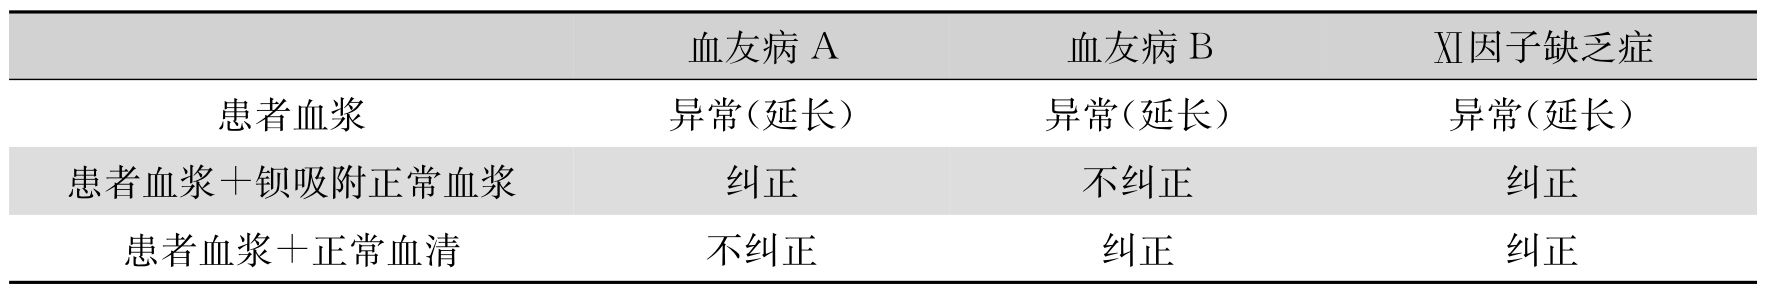
\includegraphics[width=5.90625in,height=1in]{./images/Image00206.jpg}
\end{table}

检测第Ⅷ因子和第Ⅸ因子凝血活性及抗原性很易将两者鉴别开来。

\paragraph{三、血浆凝血活酶前质缺乏症}

本病少见。

本病临床上与血友病A及血浆凝血活酶成分缺乏症的不同点是:①本病为不完全隐性常染色体基因遗传疾病,可见于两性;②本病出血症状较轻,关节积血少见;③血浆凝血时间及部分凝血活酶时间延长仅属轻度,而全血凝血时间多正常。

确诊须依靠凝血酶原消耗纠正试验、部分凝血活酶时间及凝血活酶生成纠正试验。应用实验室检查,本病难与第Ⅻ因子缺乏症鉴别(见表\ref{tab34-6})。有人提议用试管涂膜试验(glasscoating
test),可作出鉴别诊断。其原理为第Ⅻ因子缺乏所致的血浆凝血时间延长可被小量正常血清(涂膜于试管表面)所纠正,而本病则不能被纠正。更精确的试验是测定第Ⅺ因子的含量,如第Ⅺ因子降低(正常为65\%~135\%)也有诊断与鉴别诊断意义。

\paragraph{四、第Ⅻ因子缺乏症}

本病又称Hageman特性。血浆凝血时间(再钙化时间)轻度延长及一期法血浆凝血酶原时间正常,而临床上无出血症状,提示本病诊断的可能性。本病多在外科手术前作止血、凝血机制实验室检查时偶然被发现。确诊须靠凝血活酶生成纠正试验(见表\ref{tab34-6})。本病与第Ⅺ因子缺乏症鉴别见上文。

本病为常染色体隐性遗传疾病,男、女皆可罹患。

\subsubsection{116.1.2 第二阶段凝血异常}

此类疾病大多为获得性,极少为遗传性,包括低血凝血酶原血症、第Ⅶ因子缺乏症、第Ⅴ因子缺乏症及第Ⅹ因子缺乏症等四种出血性疾病。其共同特点为一期法血浆凝血酶原时间延长,但此种情况也可见于血浆纤维蛋白原缺乏症。血浆纤维蛋白原缺乏症可用血浆纤维蛋白原定量法证明。第Ⅹ因子缺乏症可用凝血活酶生成纠正试验确诊。低凝血酶原血症、第Ⅴ因子缺乏症及第Ⅶ因子缺乏症,可用凝血酶原时间纠正试验区别之(表\ref{tab34-12})。

\begin{table}[htbp]
\centering
\caption{凝血酶原时间纠正试验}
\label{tab34-12}
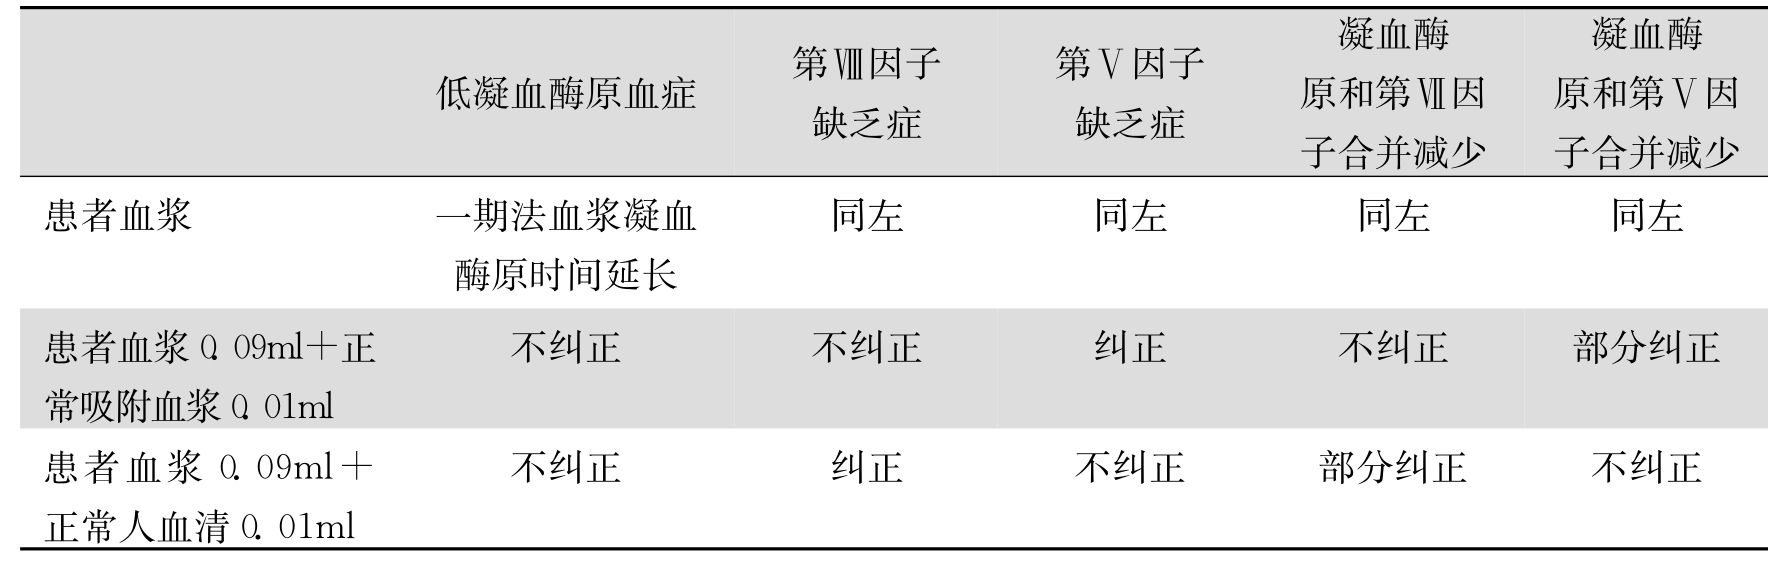
\includegraphics[width=5.9375in,height=1.875in]{./images/Image00207.jpg}
\end{table}

\paragraph{一、低凝血酶原血症}

低凝血酶原血症分为先天性(遗传性)与获得性两种。遗传性低凝血酶原血症罕见,可分两型:①全凝血酶原减少症:为常染色体隐性遗传,出血仅见于同型合子,全凝血酶原时间延长;②游离凝血酶原减少症:为常染色体显性遗传,全凝血酶原时间正常。

获得性低凝血酶原血症较为常见,可分为三型:①维生素K缺乏,见于阻塞性黄疸、吸收不良综合征、广谱抗生素疗程、新生儿出血症、双香豆素抗凝疗程等;②严重肝病;③弥散性血管内凝血。

低凝血酶原血症的出血一般发生在皮肤、肌肉及黏膜,关节内出血则极其少见。遗传性低凝血酶原血症的发病多自幼年开始,但轻症也可延至成年期发病,有时不易与获得性低凝血酶原血症相鉴别,以下两项有利于获得性低凝血酶原血症的诊断:①临床上有上述原发病的存在;②除凝血酶原缺乏外,尚有第Ⅴ、Ⅶ、Ⅷ、Ⅸ、Ⅹ等因子缺乏。

肝脏为蛋白质合成的场所,第Ⅴ、Ⅶ、Ⅸ、Ⅹ因子以及凝血酶原和纤维蛋白原主要有肝脏合成,因此,在严重肝病时主要为上述各凝血因子的减少,尤其以第Ⅴ因子减少最为显著。维生素K缺乏时,第Ⅷ、Ⅸ、Ⅹ因子和凝血酶原减少,但以第Ⅴ因子正常为特征。弥散性血管内凝血时,主要是第Ⅴ、Ⅷ因子以及凝血酶原和纤维蛋白原减少。

\paragraph{二、第Ⅴ因子缺乏症}

第Ⅴ因子(易变因子)缺乏症极少单独发生。单独发生者一般都为先天性常染色体遗传性疾病,男女均可罹患。患者凝血活酶生成纠正试验也可呈生成迟缓,有人称之为副血友病。本症国内已有病例报告。其与真性血友病实验室检查的不同点为,本病一期法血浆凝血酶原时间延长。因子Ⅴ活性及抗原测定能确定诊断。

获得性第Ⅴ因子缺乏症可见于大手术后最初数周之内,约在手术后第3天达高峰,此外,又可见于接受大量放射性物质之后,用放射性核素32磷治疗真性红细胞增多症或白血病时,也可引起第Ⅴ因子缺乏。获得性第Ⅴ因子缺乏症常与低凝血酶原血症并发,因这两种物质均受相同因素的影响。

\paragraph{三、第Ⅶ因子缺乏症}

先天性第Ⅶ因子(稳定因子)缺乏症是一种常染色体隐性遗传性疾病。常引起自发性出血(鼻出血、血肿、血尿等),或在外科手术、外伤时严重出血。此病在国内已有报告。

获得性第Ⅶ因子缺乏症可见于许多病理状态:肝脏疾病、维生素K缺乏、应用抗凝药物。此症往往与低凝血酶原血症并发。因两者的合成须有正常的肝功能。维生素K必须充分得到利用。患者的APTT、TT、BT均正常,PT延长,能被正常血清纠正,而不能被吸附血浆纠正。确诊需要测定因子Ⅶ:C及因子Ⅶ:Ag。

\paragraph{四、第Ⅹ因子缺乏症}

本病又称Stuart因子缺乏症,临床上罕见,是常染色体遗传疾病,男、女均可患病。本病除先天遗传性之外,尚可为获得性(肝病、双香豆素抗凝疗程中及淀粉样变性等)。

本病临床表现与实验室检查所见,除凝血活酶生成迟缓和凝血酶原消耗不良以外,与第Ⅶ因子缺乏症甚为相似。本病可有皮肤、黏膜及关节出血。实验室检查一期法血浆凝血酶原时间延长能被陈旧血浆所纠正,而不被吸附血浆所纠正,蛇毒时间延长,强烈提示本病的可能性。确诊须测定因子Ⅹ活性及抗原。

本病一期法血浆凝血酶原时间延长,须与第Ⅶ因子缺乏症区别。本病蛇毒时间延长而第Ⅶ因子缺乏时则正常。本病的凝血活酶生成纠正试验结果与第Ⅸ因子缺乏相同,但本病同时有一期法血浆凝血酶原时间延长,而第Ⅸ因子缺乏则正常。

\subsubsection{116.1.3 第三阶段凝血异常}

纤维蛋白原缺乏症

纤维蛋白原缺乏症的实验室检查特点是凝血酶时间延长、血浆纤维蛋白原测定含量下降。

纤维蛋白原缺乏症可分为先天性或获得性,但如血浆纤维蛋白原完全缺乏,一般为先天性。先天性无纤维蛋白原血症国内未见报告。获得性纤维蛋白原缺乏症可见于重症肝损害、弥散性血管内凝血以及继发性纤维蛋白溶解症。

\subsubsection{116.1.4 维生素K缺乏症}

维生素K缺乏引起第Ⅱ、Ⅶ、Ⅸ、Ⅹ以及蛋白C和蛋白S活性的降低。其原因包括先天性维生素K依赖性凝血因子缺乏症、食物性维生素K缺乏症、胆汁阻塞综合征和吸收不良综合征、肝脏疾病、双香豆素类作用以及鼠药中毒、某些中草药或抗生素使用等。除原发病的表现外,主要表现为皮肤、黏膜出血、内脏出血、外伤或手术后伤口出血、新生儿出血症。

实验室检查PT、APTT延长,FⅦ、FⅨ、FⅩ、凝血酶原抗原及活性降低。

诊断要点:存在引起维生素K缺乏的基础疾病;皮肤、黏膜及内脏轻、中度出血;PT、APTT延长,FⅦ、FⅨ、FⅩ、凝血酶原抗原及活性降低;维生素K治疗有效。

\subsubsection{116.1.5 异常蛋白血症}

此组疾病包括巨球蛋白血症、冷球蛋白血症、多发性骨髓瘤及淀粉样变性等。此组疾病的共同特点为血浆中出现M蛋白。M蛋白与凝血因子结合,使后者灭活,为出血的主要原因之一。

\paragraph{一、原发性巨球蛋白血症}

又名Waldenstrom巨球蛋白血症。是一种原因未明,源自B淋巴细胞,具有合成和分泌IgM能力的淋巴样浆细胞恶性增殖性疾病,男女发病率大致相等,多见于中、老年人,起病隐匿。以贫血,肝、脾、淋巴结肿大,高黏滞综合征,出血倾向,中枢及周围神经系统症状为特征。

临床上有出血倾向。血中淋巴细胞增多及血沉增快时,提示本病诊断的可能性。

本病临床上主要有以下两种病征:

\subparagraph{1.巨球蛋白增多所致的病征}

①血浆黏稠度增加,引起血循环障碍,表现为乏力、气短(脑及体循环障碍);轻瘫、意识障碍(脑循环障碍);视力障碍,眼底出血渗出、静脉曲张及淤血(眼底循环障碍)。②有些巨球蛋白具有冷凝集作用的性质,可能是一种巨冷球蛋白(macrocryoglobulin),能引起雷诺现象及冷荨麻疹。③巨球蛋白可直接损伤血管壁,与凝血因子结合并干扰血小板功能,可有出血倾向。④血沉增快。

\subparagraph{2.淋巴样浆细胞增生所致的病征}

①骨髓淋巴细胞增高,淋巴浆细胞样细胞和组织嗜碱细胞也增多。②外周血全血细胞减少,淋巴细胞增多。③肝、脾、淋巴结肿大。

实验室检查:血浆球蛋白在50g/L以上为诊断本病的线索。超速离心法及免疫电泳从血浆中检出大量巨球蛋白(19S,IgM
10~120g/L)可以确诊。

血清蛋白电泳巨球蛋白呈基底部狭窄和高而尖锐的顶峰的图形,即单克隆蛋白(M球蛋白)图形。M球蛋白也见于多发性骨髓瘤和良性单克隆丙种球蛋白病(benign
monoclonal gammopathy)。

本病的诊断依据是:①患者年龄多在60岁以上,伴原因不明的贫血。②骨髓与淋巴结内有淋巴细胞、浆细胞,特别是淋巴样浆细胞浸润。③血清中出现大量单克隆IgM,其浓度超过10g/L。④血沉加快,多有高黏度血及眼底改变(出血或静脉扩张)。①、④两项可作为重要的辅助诊断依据。

诊断原发性巨球蛋白血症时,尚需除外继发性巨球蛋白血症,后者继发于淋巴细胞型白血病、恶性淋巴瘤、癌、结缔组织病、慢性感染及肝硬化等,这些疾病也可有巨球蛋白增多,但很少超过血清蛋白的15\%,且有原发病存在。

\paragraph{二、意义未明单克隆γ球蛋白症(monoclonal gammopathy of undetermined}
significance,MGUS)

患者血液和(或)尿液中出现单克隆免疫球蛋白式轻链,能除外恶性浆细胞病或淋巴增强性疾病及其他能够引起单克隆免疫球蛋白增高的疾病,其自然病程、预后和转归暂时无法确定的疾病状态。本病又名“良性”高丙种球蛋白血症或良性单克隆丙种球蛋白病,病因未明。临床和实验室特点:①无明显的临床症状,也无骨髓的损害征,偶可有轻微出血倾向;②血液中出现单克隆免疫球蛋白,但含量<30g/L;③骨髓浆细胞数增多,但比例<10\%。

实验室检查是发现本病的主要手段,表现为血清球蛋白增高,血清蛋白电泳呈现浓染的条带,大多位于γ区,少数分布在β区,极少数分布在α\textsubscript{2}
区。

大多数病情保持长期稳定,部分患者经过若干年后发展为多发性骨髓、原发性淀粉样变、巨球蛋白血症等恶性浆细胞病。个别患者可能是恶性淋巴增强性疾病的早期,因此所有患者均需长期随访。

本病需与原发性巨球蛋白血症及多发性骨髓瘤相区别。虽然本病与多发性骨髓瘤有相似的电泳蛋白图形,但无骨质破坏区,骨髓浆细胞计数下降(或轻度增多),副蛋白的浓度1~2年内无改变,可与多发性骨髓瘤相区别。

\protect\hypertarget{text00266.html}{}{}

\subsection{116.2 抗凝及纤维蛋白溶解异常}

\subsubsection{一、获得性凝血抑制物}

获得性凝血抑制物是一些能够直接中和血液中凝血蛋白或干扰凝血反应的病理性大分子成分,多以抗体形式出现。最常见的获得性凝血抑制物是抗磷脂抗体,包括狼疮型抗凝物和抗心磷脂抗体,继发于系统性红斑狼疮等自身免疫性疾病;获得性因子Ⅷ抑制物常见于血友病A因子Ⅷ替代治疗后。出血患者实验室检查显示全血凝血时间延长、血浆凝血时间延长,一般提示凝血因子缺乏或抗凝物质所致出血性疾病的可能性,作抗凝物质检定试验可区别之。

根据抗凝物质的作用和发生机制的不同,获得性抗凝物质可分为:①阻止凝血活酶形成的抗凝物质,如发生在血友病患者反复接受输血之后,系统性红斑狼疮,妊娠,老年人等;②对已形成的凝血活酶有阻抑作用的抗凝物质,可见于系统性红斑狼疮;③类肝素作用的抗凝物质,可见于系统性红斑狼疮、肝病、老年人、恶性肿瘤等。

1.阻止活动性凝血活酶形成的抗凝物质凝血酶原在凝血时的消耗受到显著的障碍。采血时加入大量的凝血活酶可部分纠正上述障碍。一期法血浆凝血酶原时间正常或略延长,凝血活酶生成纠正试验的结果显示很少活动性凝血活酶形成。

2.存有对抗已经形成的活动性凝血活酶的抗凝物质凝血酶原消耗仅受轻度障碍,但一期法血浆凝血酶原时间延长,加入大量组织凝血活酶后,仅能得到部分纠正。

3.存有类肝素作用的抗凝物质凝血过程中所有阶段多少都要受到影响:①血浆凝血酶原的活动度轻度减低;②凝血酶原消耗也受障碍;③血浆抗凝血酶浓度增高,加硫酸鱼精蛋白或甲苯胺蓝后,这些患者的止血障碍完全被纠正。

通常的抗凝疗法时所应用的抗凝剂,如肝素或双香豆素,如用量过大,也可引起出血。肝素可使全血凝血时间延长,双香豆素可使一期法血浆凝血时间延长。在施行抗凝疗法时,应作上述的实验室检查作为确定剂量或断续给药的参考。

\subsubsection{二、原发性纤维蛋白溶解症}

在病理情况下,纤维蛋白溶酶活性显著增强,超过了抗纤维蛋白溶解系统的功能,导致纤维蛋白或纤维蛋白原的过度分解,往往引起出血现象。原发性纤维蛋白溶解症的病因与发病机制大致归纳为:①前纤维蛋白溶酶活化素(plasminogen
activator)增多,可见于恶性肿瘤、手术、创伤、缺氧、败血症、休克及链激酶(streptokinase)等药物疗程中。②抗纤维蛋白溶解系统功能不足,例如失代偿性肝硬化。③与纤维蛋白溶酶有相同作用的蛋白分解酶的释放,例如晚期白血病。

在上述基本疾病的基础上发生出血现象,血不凝或凝固以后迅速溶解,提示原发性纤维蛋白溶解症。

前纤维蛋白溶酶活化素与蛋白分解酶可能具有凝血活性,也可引起血管内凝血。

原发性纤维蛋白溶解症的血液实验室检查有以下特点:血块回缩试验回缩时间延长。血块松脆,凝血酶时间延长,凝血酶原时间延长,纤维蛋白原定量减少,第Ⅴ因子、第Ⅷ因子中度减少,纤维蛋白(原)降解产物(FDP、Bρ1-42、Bρ15-42等)增高。前纤维蛋白溶酶减少及优球蛋白溶解时间缩短,后者有确诊的意义。

弥散性血管内凝血与原发性纤维蛋白溶解症都有血管内凝血和纤维蛋白(原)溶解。从治疗角度对两者进行鉴别诊断有一定意义。前者为抗凝疗法的适应证,6-氨基己酸慎用;后者为应用6-氨基己酸的适应证,抗凝疗法慎用。

\protect\hypertarget{text00267.html}{}{}

\subsection{116.3 复合性止血机制异常}

\subsubsection{一、血管性血友病}

血管性血友病(von Willebrand
disease,vWD)包括遗传性血管性血友病(cvWD)和获得性血管性血友病(avWD)。cvWD是VWD是常染色体显性遗传。avWD最常见的原因为自身性疾病、非霍奇金淋巴瘤(NHL)、多发性骨髓瘤(MM)、实体瘤、某些药物(丙戊酸钠、环丙沙星)。

vWD是由于血浆中与Ⅷ因子相关的vWF在结构和(或)功能上异常所致。皮肤黏膜出血,特别是轻微创伤后持续出血是VWD患者特征性的临床表现。

实验室检查包括出血时间延长、活化的部分凝血活酶时间(APTT)延长、阿司匹林耐量试验异常;确诊靠瑞斯托霉素辅因子检测,vWF抗原测定和Ⅷ因子水平测定。vWD多聚体分析有助于vWD分型诊断。

\subsubsection{二、弥散性血管内凝血}

弥散性血管内凝血(disseminatedintravascularcoagulation,DIC)是一种病理过程,发生在许多疾病基础上,由不同原因引起,是以全身性血管内凝血系统被激活为特征的综合征,可引起微血管系统损伤。常导致广泛出血,严重时可导致器官功能衰竭。

诱发DIC的基础疾病种类如下:

\paragraph{(一)组织损伤}

1.产科重症妊娠中毒症,胎盘早期剥离,羊水栓塞,死胎滞留,感染性流产,子宫破裂,葡萄胎,刮宫等。

2.外科广泛性手术,血管外科手术,挤压综合征,大面积烧伤,前列腺手术,胰腺手术。

3.肿瘤 前列腺癌,支气管癌,甲状腺癌,绒毛膜上皮癌。各种黏液腺癌的广泛浸润和转移。

4.白血病 各型急性白血病,特别是早幼粒细胞型。

5.化学药物治疗之后。

\paragraph{(二)内皮损伤}

1.革兰氏阴性细菌败血症 脑膜炎双球菌、大肠杆菌、铜绿假单胞菌、肺炎克雷伯菌、阴沟肠杆菌。

2.革兰氏阳性细菌败血症 肺炎双球菌、金黄色葡萄球菌、肠球菌。

3.病毒血症 病毒性心肌炎、病毒性肺炎、病毒性脑膜(脑)炎等。

4.长期低血压。

5.其他 中暑、巨血管瘤。

\paragraph{(三)血小板或红细胞损伤}

1.免疫性 暴发型紫癜、系统性红斑狼疮等。

2.溶血性 血型不合溶血、输血反应、溶血性贫血、微血管病性溶血性贫血等。

3.疟疾。

\paragraph{(四)单核-吞噬细胞系统损伤}

1.肝损害 急性暴发型肝炎、失代偿性肝硬化等。

2.脾切除后。

凡在上述疾病中,出现低血压、出血、少尿、尿闭、恶心、呕吐、腹痛、腹泻、背痛、呼吸困难和发绀等症状,提示弥散性血管内凝血的可能。

临床上弥散性血管内凝血主要特点为:①出血不止与血液不凝(或血凝减慢),或血凝后的血块又发生溶解,出血常发生的皮肤、黏膜、内脏、手术切口、外伤创面等部位,皮肤紫斑与大片瘀斑,在注射或手术部位易发生持续性渗血。这是DIC的一个很特殊的表现。内脏出血表现咯血、呕吐、血便、血尿。②栓塞现象,主要是微循环的栓塞,可有休克、少尿、无尿及急性肾衰竭,偶有大血管栓塞,如脑动脉栓塞、肺栓塞及多发性静脉栓塞等;DIC的栓塞往往是全身性的。③微血管病性溶血。主要表现为贫血,很少像急性溶血那样出现发热、黄疸或血红蛋白尿。这是由于DIC时微血栓的形成可使红细胞变形与碎裂导致溶血。④实验室检查:血小板计数<100×
10\textsuperscript{9}
/L或呈进行性下降;血浆纤维蛋白原浓度<1.5g/L,或呈进行性下降;3P试验阳性或血浆FDP>20mg/L;凝血酶原时间缩短或延长3秒以上,肝病延长5秒以上,或APTT缩短或延长10秒以上。2001年国际血栓与止血协会提出的积分系统获得了大多数学者的认可。

血管内凝血的过程中,由于机体一种代偿防御反应,或由于凝血酶直接激活前纤维蛋白溶酶,可引起继发性纤维蛋白溶解,此时出血更为严重,优球蛋白溶解时间缩短。临床上须与原发纤维蛋白溶解症及重症肝炎相区别(表\ref{tab34-13}和表\ref{tab34-14})。

DIC与血栓性血小板减少性紫癜(TTP)鉴别:TTP有血小板减少和微血管病性溶血而出现的贫血和红细胞碎片以及微血栓导致的肾损害,神经精神异常等与DIC相似。但TTP患者的神经精神异常症状变化不定,发热多是TTP患者常见的首发表现。TTP患者无纤溶亢进,因此无纤维蛋白原进行性下降,FDP动态上升及D-二聚体升高等与DIC的显著区别。

DIC与血小板减少性紫癜(ITP)鉴别:虽两者均有血小板减少及出血表现,但ITP出血以皮肤紫癜为主要表现。ITP实验室检查除血小板计数明显下降外,无凝血因子减少及纤溶亢进等指标异常。

\begin{table}[htbp]
\centering
\caption{弥散性血管内凝血与原发纤维蛋白溶解症的鉴别}
\label{tab34-13}
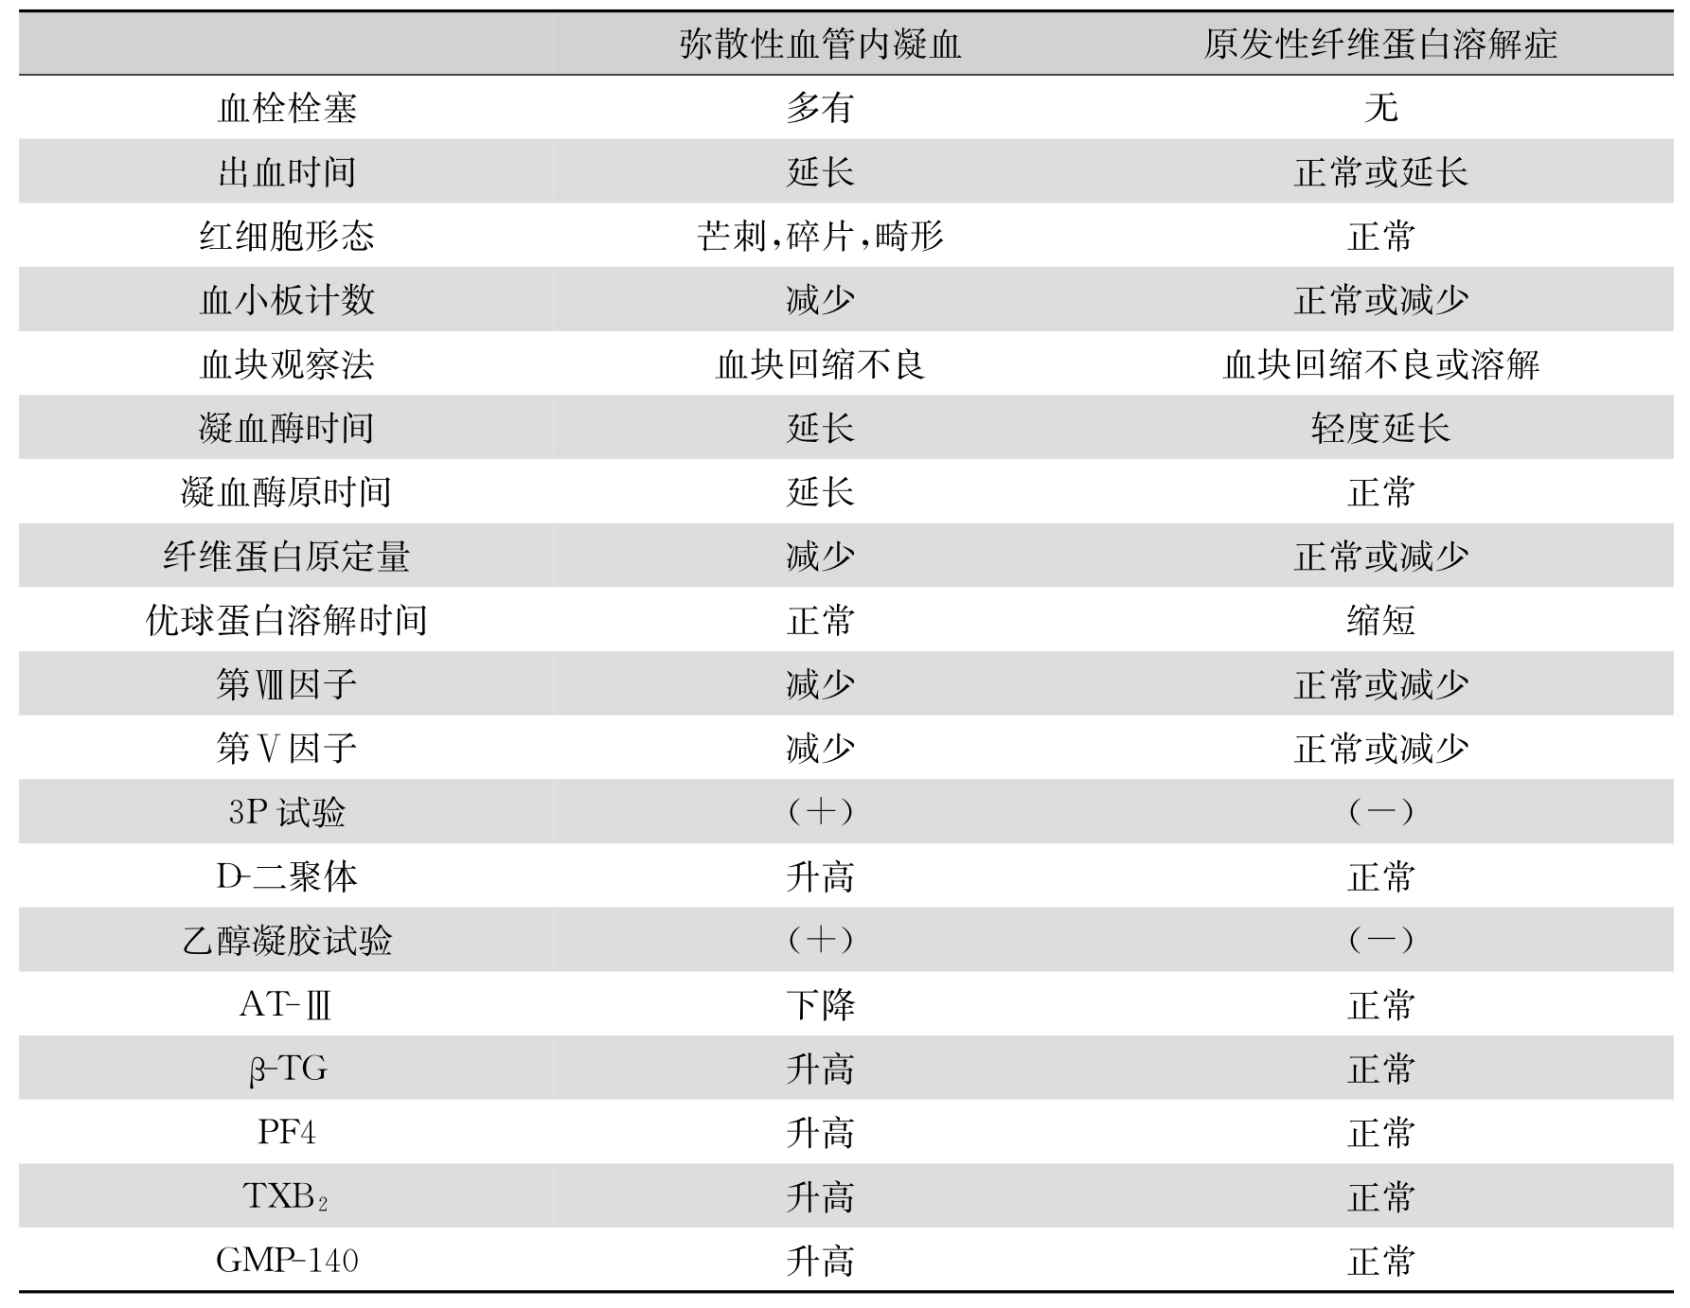
\includegraphics[width=5.9375in,height=4.59375in]{./images/Image00208.jpg}
\end{table}

\begin{table}[htbp]
\centering
\caption{DIC与重症肝类的鉴别}
\label{tab34-14}
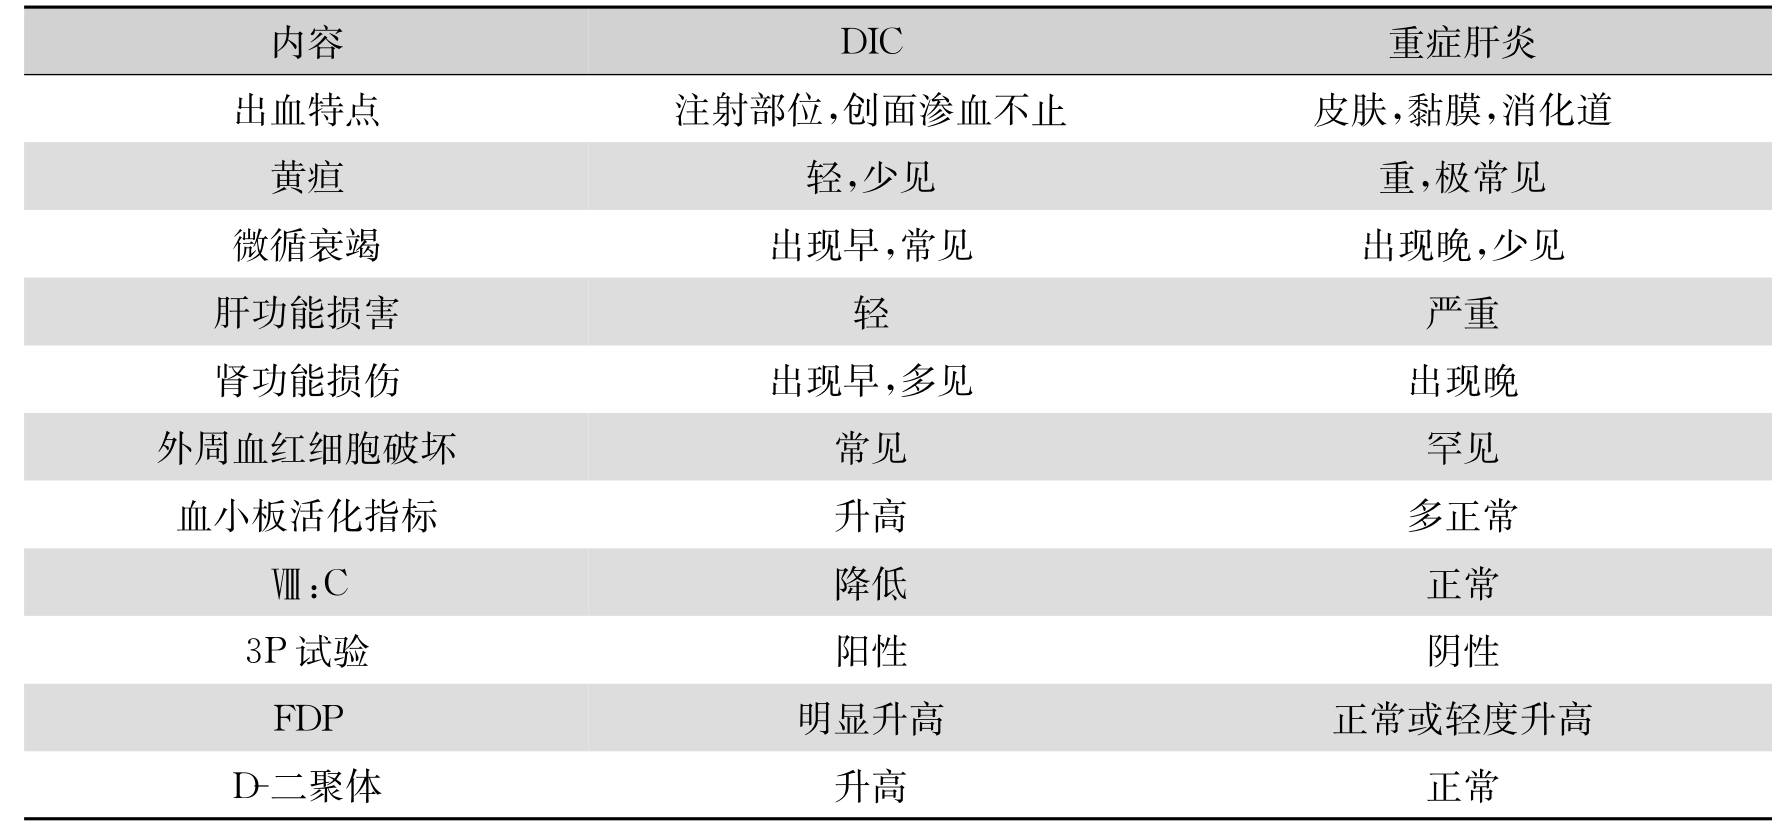
\includegraphics[width=5.9375in,height=2.78125in]{./images/Image00209.jpg}
\end{table}

\protect\hypertarget{text00268.html}{}{}

\section{参考文献}

1.易彦,等.遗传性出血性毛细血管扩张症的研究进展.国外医学输血及血液学分册,2004,27(1):27-29

2.齐薇薇,等.成人过敏性紫癜35例临床分析.中国实用内科杂志,2009,29(2):147-149

3.张安忠,等.成人腹型过敏性紫癜的临床和内镜特征.中华消化内镜杂志,2005,22(2):108-110

4.杨海燕,等.遗传性巨大血小板病的研究进展.国外医学输血及血液学分册,2005,28(5):459-462

5.中华医学会血液学分会血栓与止血学组.成人原发免疫性血小板减少症诊治的中国专家共识(修订版).中华血液学杂志,2011,32(3):214-216

6.Rawi Hazzan,et al.Risk factors for future development of systemic
lupus erythematosus in children with lidiopathic thrombocytopenic
purpura.Pediatr Blood Cancer,2006,47:657-659

7.Roberto Stasi.Idiopathic thrombocytopenic purpura:Current concepts in
pathophysiology and management. Thromb Haemost,2008,99:4-13

8.董恂玮,等.84例成人Evans综合征临床资料分析.中华血液学杂志,2010,31(7):475-477

9.邓明扬,等.血栓性血小板减少性紫癜研究进展.国际输血及血液学杂志,2010,33(2):122-125

10.许洪志,等.血栓性血小板减少性紫癜8例临床分析.临床血液学杂志,2003,16(2):85-86

11.徐亮,等.系统性红斑狼疮合并重症血小板减少的临床特征.中华风湿病学杂志,2003,7(12):749-751

12.中华医学会血液学分会.血栓与止血学血友病诊断与治疗中国专家共识.中华血液学杂志,2011,32(3):212-213

13.王兆铖.血友病诊治的进展与展望.临床血液学杂志,2004,17(2):63

14.丁凯阳,等.先天性纤维蛋白原减少症患者伴有血小板连结蛋白的增高.中华血液学杂志,2002,23(3):143-146

15.郑昌成,等.获得性维生素K依赖性凝血因子缺乏.中华血液学杂志,2010,31(5):351-352

16.姜波,等.弥散性血管内凝血积分系统及其评价.中华血液学杂志,2007,28(12):853-855

\protect\hypertarget{text00269.html}{}{}

